\chapter{Ergebnisse}

\section{Klassifizierung zwischen Tumor und no Tumor}

\subsection{Hyperparameter}
Die fünf Trainingsdurchläufen (Runs) mit den niedrigsten Validation Loss wird in der Abbildung \ref{fig:val_loss notu-tu} dargestellt.
\begin{figure}[H]
  \centering
  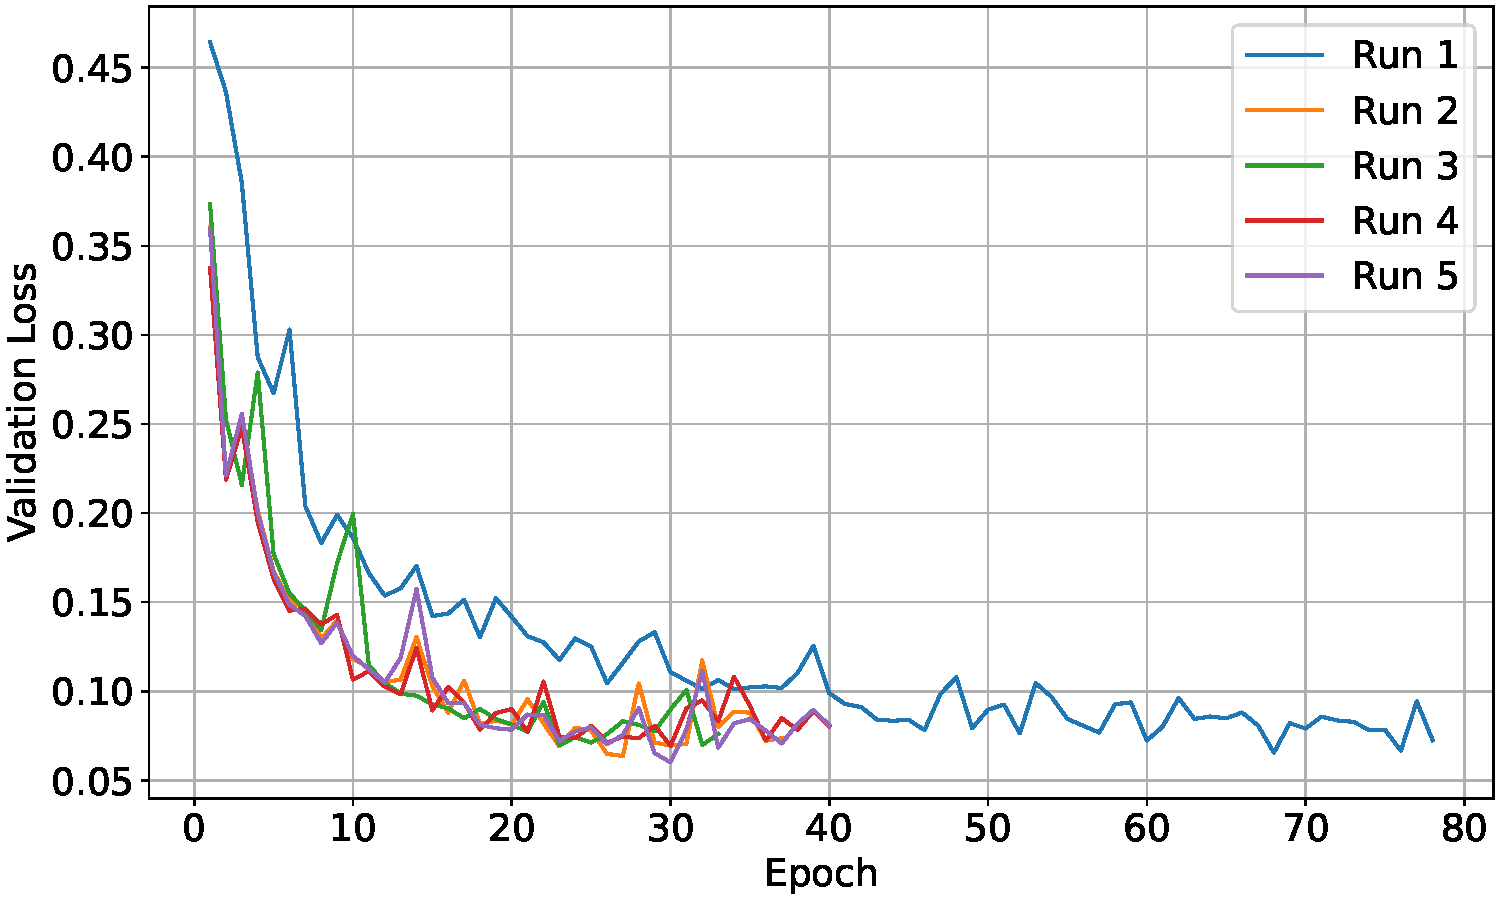
\includegraphics[scale=0.4]{plots/Val_loss_noTu_Tu.pdf}
  \caption{Verlauf des validation loss bei der Verwendung verschiedener Hyperparameter.}
  \label{fig:val_loss notu-tu}
\end{figure}
%\vspace{-1.5em}
In der Tabelle \ref{tab:hyperp notu-tu} sind die dabei verwendeten Hyperparameter, sowie die aufgenommen Metriken zu finden. 
\begin{table}[H]
    \centering
    \resizebox{\textwidth}{!}{%
        \begin{tabular}{cccccccc}
            \toprule
            Runs & Batch Größe & Lernrate & Dropout & validation loss & Accuracy/$\%$ & Sensitivity & Specificity \\
            \midrule
            1 & 128 & 0.005  & 0.55 & 0.072539 & 97.53231 & 0.97967 & 0.96774 \\
            2 & 128 & 0.0005 & 0.5  & 0.073672 & 98.00235 & 0.98706 & 0.96774 \\
            3 & 16  & 0.0001 & 0.5  & 0.076007 & 97.88484 & 0.97597 & 0.98387 \\
            4 & 128 & 0.0005 & 0.4  & 0.080399 & 97.76733 & 0.97782 & 0.97742 \\
            5 & 128 & 0.0005 & 0.5  & 0.080853 & 97.64982 & 0.98706 & 0.95806 \\
            \bottomrule
        \end{tabular}
    }
  \caption{Die fünf Runs mit dem niedrigsten validation loss sowie deren verwendete Hyperparameter und aufgezeichnete Metriken.}
  \label{tab:hyperp notu-tu}
\end{table}
%\vspace{-1em}
Die Werte der Accuracy, Sensitivity und Specificity liegen dicht bei einander und schwanken nur geringfügig.
Aufgrund dessen werden die Hyperparameter des ersten Runs für die weiteren Trainingsdurchläufen verwendet.

\subsection{Reduzierung der Trainingsdaten}

Die aufgenommen Metriken werden gegen die verwendeten Anzahl an Trainingsdaten aufgetragen. 
Dies wird in der Abbildung \ref{fig:reduzierung_trainingsdaten} gezeigt.
\begin{figure}[htbp]
  \centering
  \begin{subfigure}[b]{0.48\textwidth}
    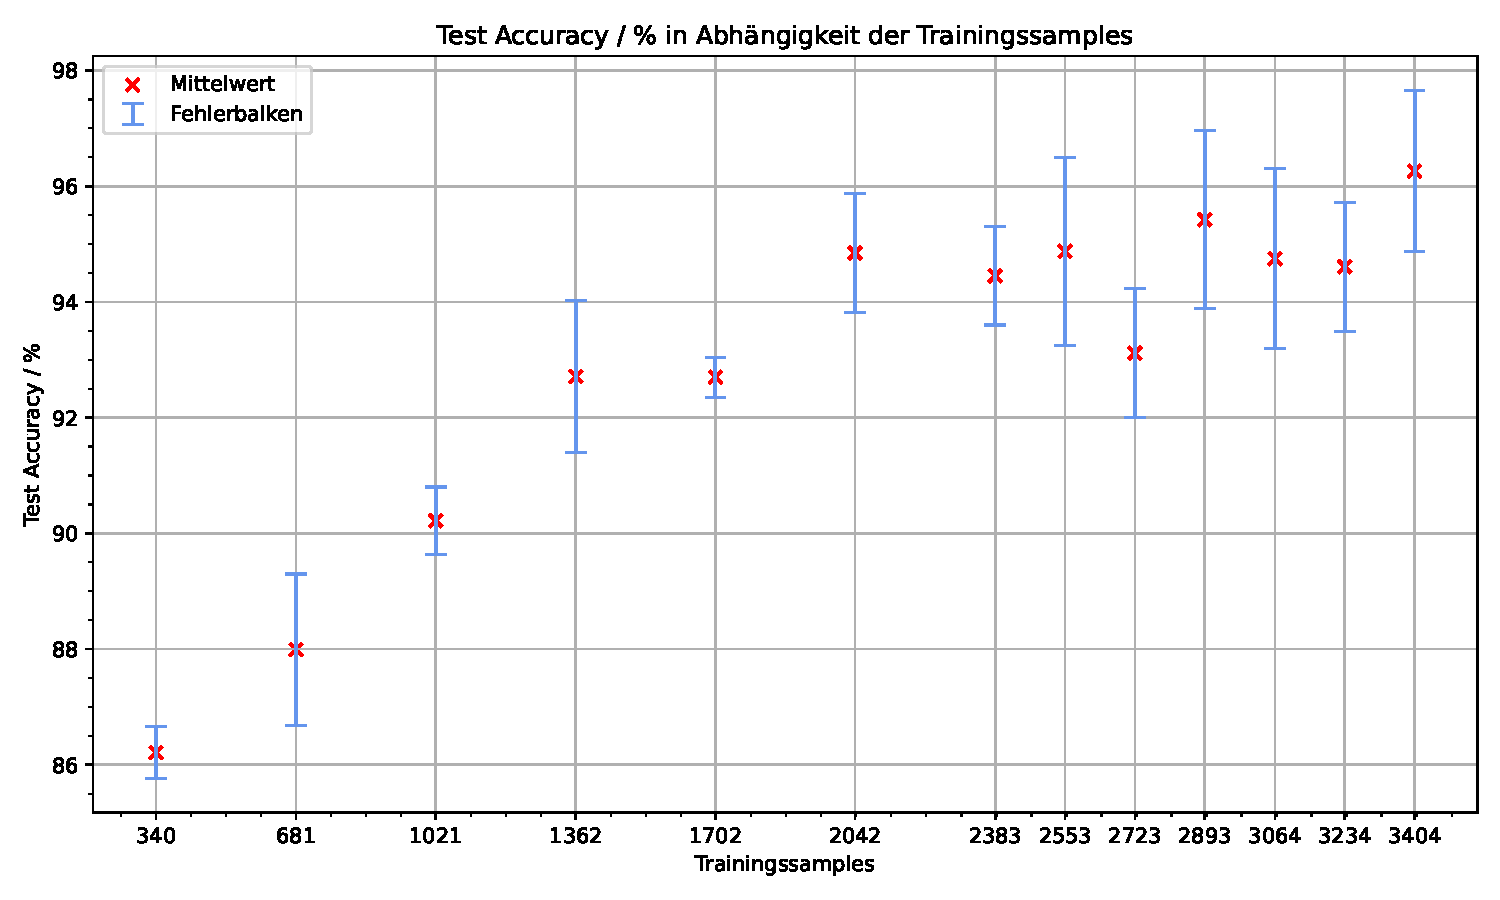
\includegraphics[width=\textwidth]{plots/2-Messungen-noTu-Tu_Accuracy_mean.pdf}
    \caption{Accuracy}
    \label{fig:reduzierung_accuracy}
  \end{subfigure}
  \begin{subfigure}[b]{0.48\textwidth}
    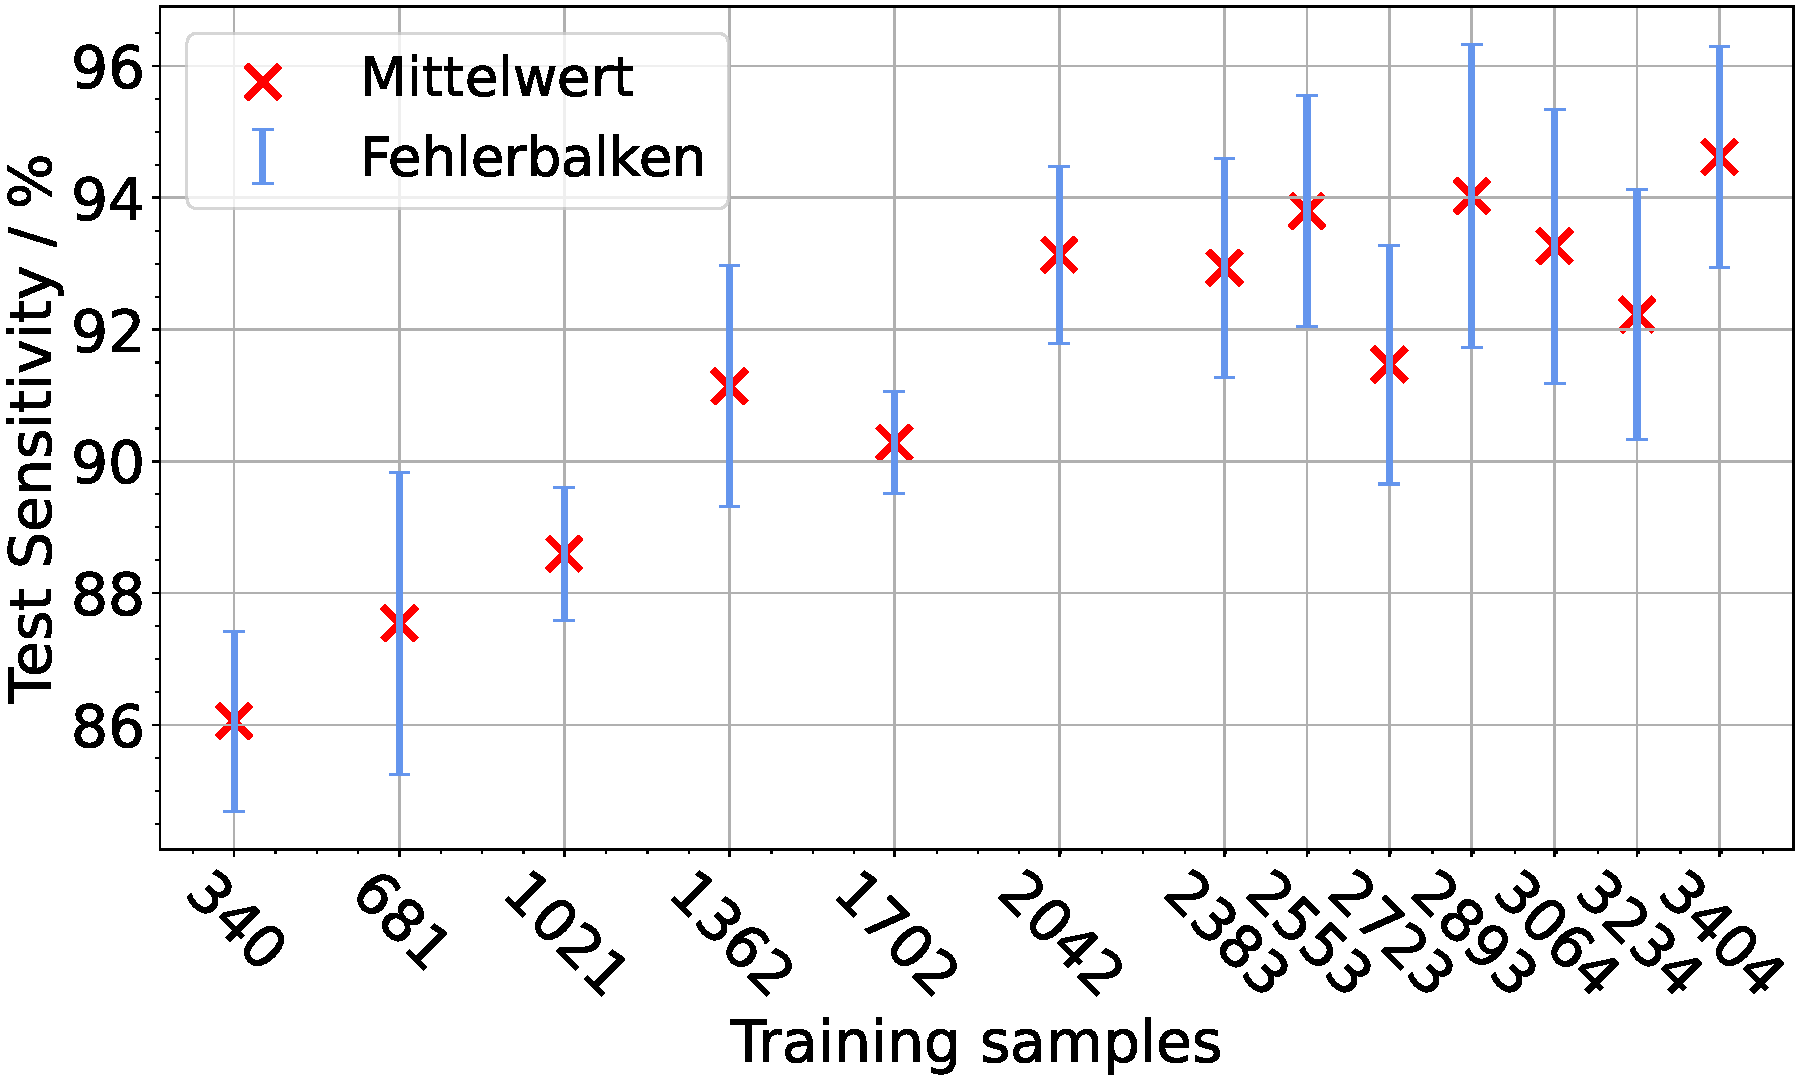
\includegraphics[width=\textwidth]{plots/2-Messungen-noTu-Tu_Sensitivity_mean.pdf}
    \caption{Sensitivity}
    \label{fig:reduzierung_sensitivity}
  \end{subfigure}
  \begin{subfigure}[b]{0.48\textwidth}
    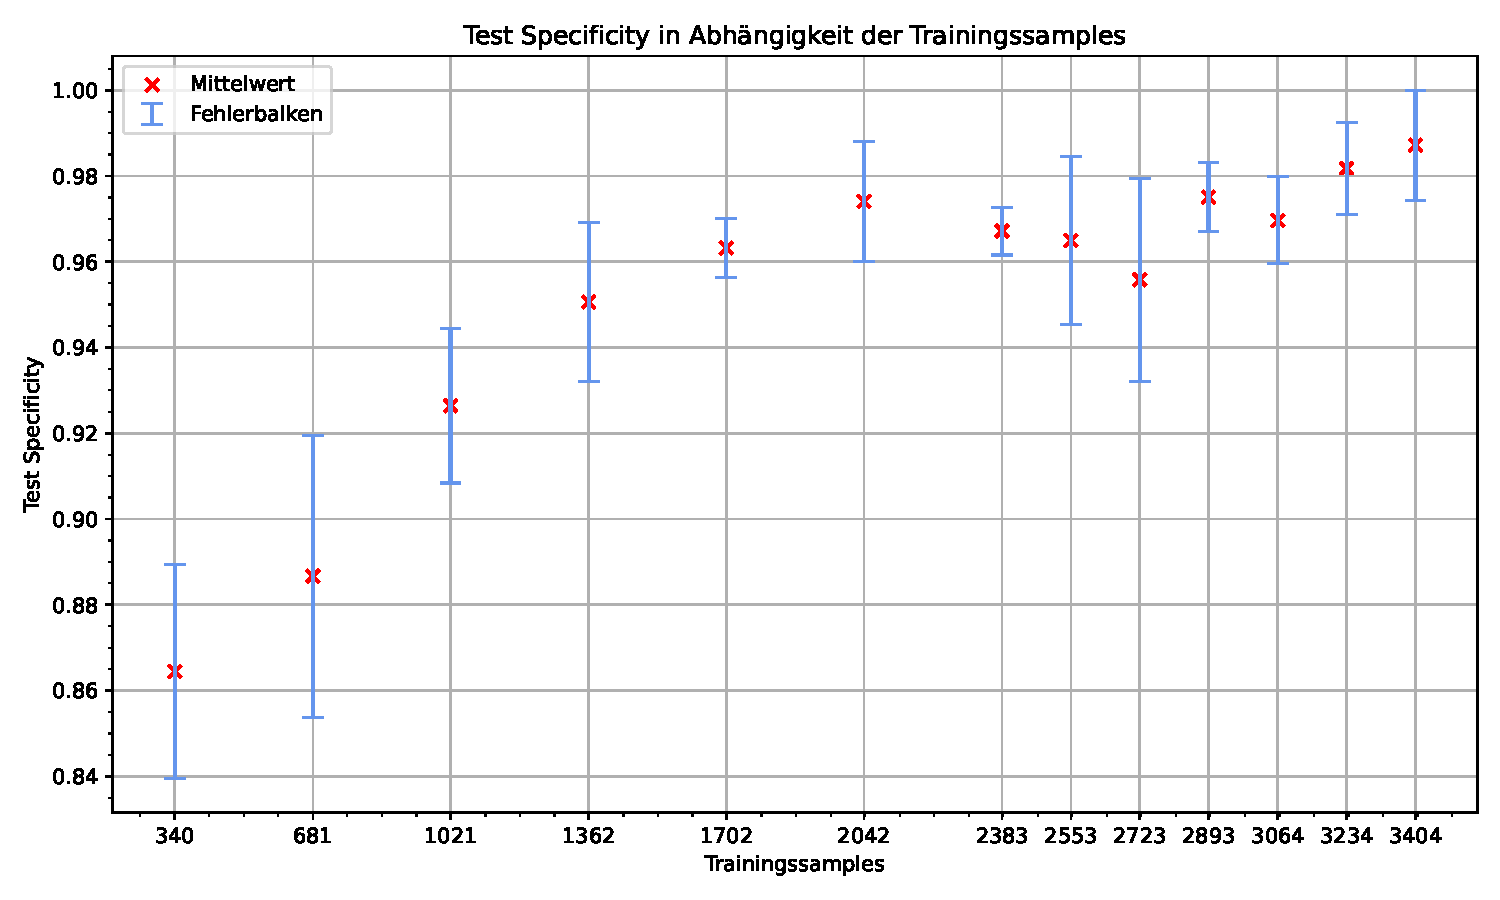
\includegraphics[width=\textwidth]{plots/2-Messungen-noTu-Tu_Specificity_mean.pdf}
    \caption{Specificity}
    \label{fig:reduzierung_specificity}
  \end{subfigure}
  \caption{Aufgenommene Metriken in Abhängigkeit der Verwendeten Trainingsdaten.}
  \label{fig:reduzierung_trainingsdaten}
\end{figure}

Die dazugehörigen Werte sind in der Tabelle \ref{tab:reduzierung_trainingsdaten} aufgelistet.
\begin{table}[htbp]
    \centering
        \begin{tabular}{cccc}
            \toprule
            Training sample & Accuracy & Sensitivity & Specificity\\
            \midrule
            340  & $86.2117 \pm 0.4428$ & $0.8606 \pm 0.0137 $ & $0.8644 \pm 0.0249$\\
            681  & $87.9921 \pm 1.3057$ & $0.8754 \pm 0.0229 $ & $0.8867 \pm 0.0329$\\
            1021 & $90.2176 \pm 0.5832$ & $0.8860 \pm 0.0101 $ & $0.9264 \pm 0.0180$\\
            1362 & $92.7102 \pm 1.3106$ & $0.9114 \pm 0.0183 $ & $0.9506 \pm 0.0186$\\
            1702 & $92.7003 \pm 0.3452$ & $0.9028 \pm 0.0078 $ & $0.9632 \pm 0.0068$\\
            2042 & $94.8467 \pm 1.0316$ & $0.9314 \pm 0.0134 $ & $0.9741 \pm 0.0140$\\
            2383 & $94.4510 \pm 0.8502$ & $0.9294 \pm 0.0166 $ & $0.9672 \pm 0.0056$\\
            2553 & $94.8764 \pm 1.6231$ & $0.9380 \pm 0.0175 $ & $0.9649 \pm 0.0196$\\
            2723 & $93.1157 \pm 1.1163$ & $0.9147 \pm 0.0181 $ & $0.9558 \pm 0.0237$\\
            2893 & $95.4204 \pm 1.5352$ & $0.9403 \pm 0.0230 $ & $0.9751 \pm 0.0080$\\
            3064 & $94.7478 \pm 1.5545$ & $0.9327 \pm 0.0208 $ & $0.9696 \pm 0.0102$\\
            3234 & $94.6093 \pm 1.1125$ & $0.9223 \pm 0.0190 $ & $0.9817 \pm 0.0108$\\
            3404 & $96.2611 \pm 1.3948$ & $0.9462 \pm 0.0167 $ & $0.9872 \pm 0.0128$\\ 
            \bottomrule
        \end{tabular}
  \caption{Mittelwert und Standardabweichung der Metriken beim Reduzieren der Trainingsgröße.}
  \label{tab:reduzierung_trainingsdaten}
\end{table}
Da die Accuracy bei einer Datengröße von 2723 Bildern sinkt, wurde zusätzlich das Training bei 
2553, 2893 und 3234 Bildern durchgeführt, um den Verlauf genauer zu untersuchen.
Die aufgenommen Metriken besitzen ihren maximal wert, bei 3404 und somit $\qty{100}{\%}$ des verwendete Datensatzes.
Am geringsten sind die Werte bei 340 Bildern.
Mit zunehmender Datenmenge steigen die Werte der Metriken.
Ab einer verwendet Menge von 2042 Daten nähren sich die Werte einem Plateau.
Für die Accuracy liegt das Plateau bei ungefähr $\qty{95}{\%}$, bei der Sensitivity ca. $0.93$ und bei der Specificity liegt die Sättigung bei ungefähr $0.98$. 
Es treten noch geringfügige Schwankungen auf.

\subsection{Augmentation}

\begin{figure}[H]
  \centering
  \begin{subfigure}[b]{0.48\textwidth}
    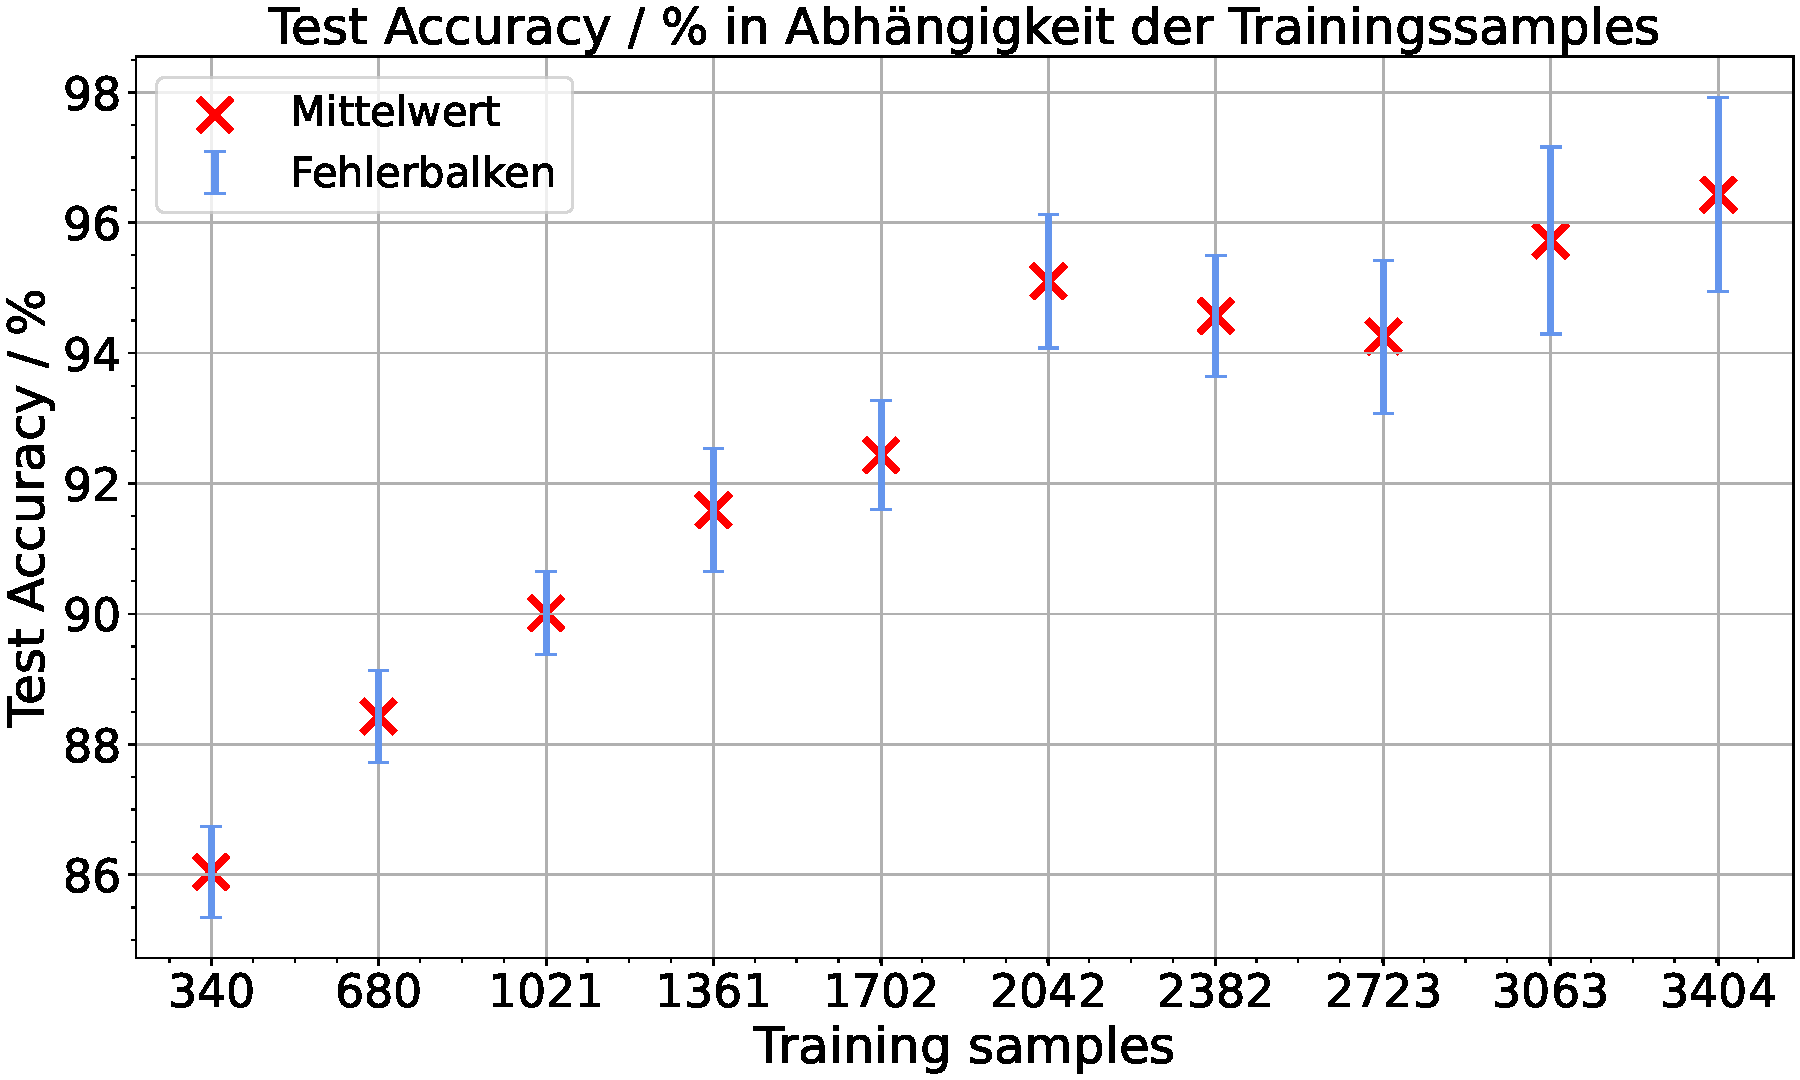
\includegraphics[width=\textwidth]{plots/Augm-Messungen-noTu-Tu_Accuracy_mean.pdf}
    \caption{Accuracy}
    \label{fig:augmentation_accuracy}
  \end{subfigure}
  \begin{subfigure}[b]{0.48\textwidth}
    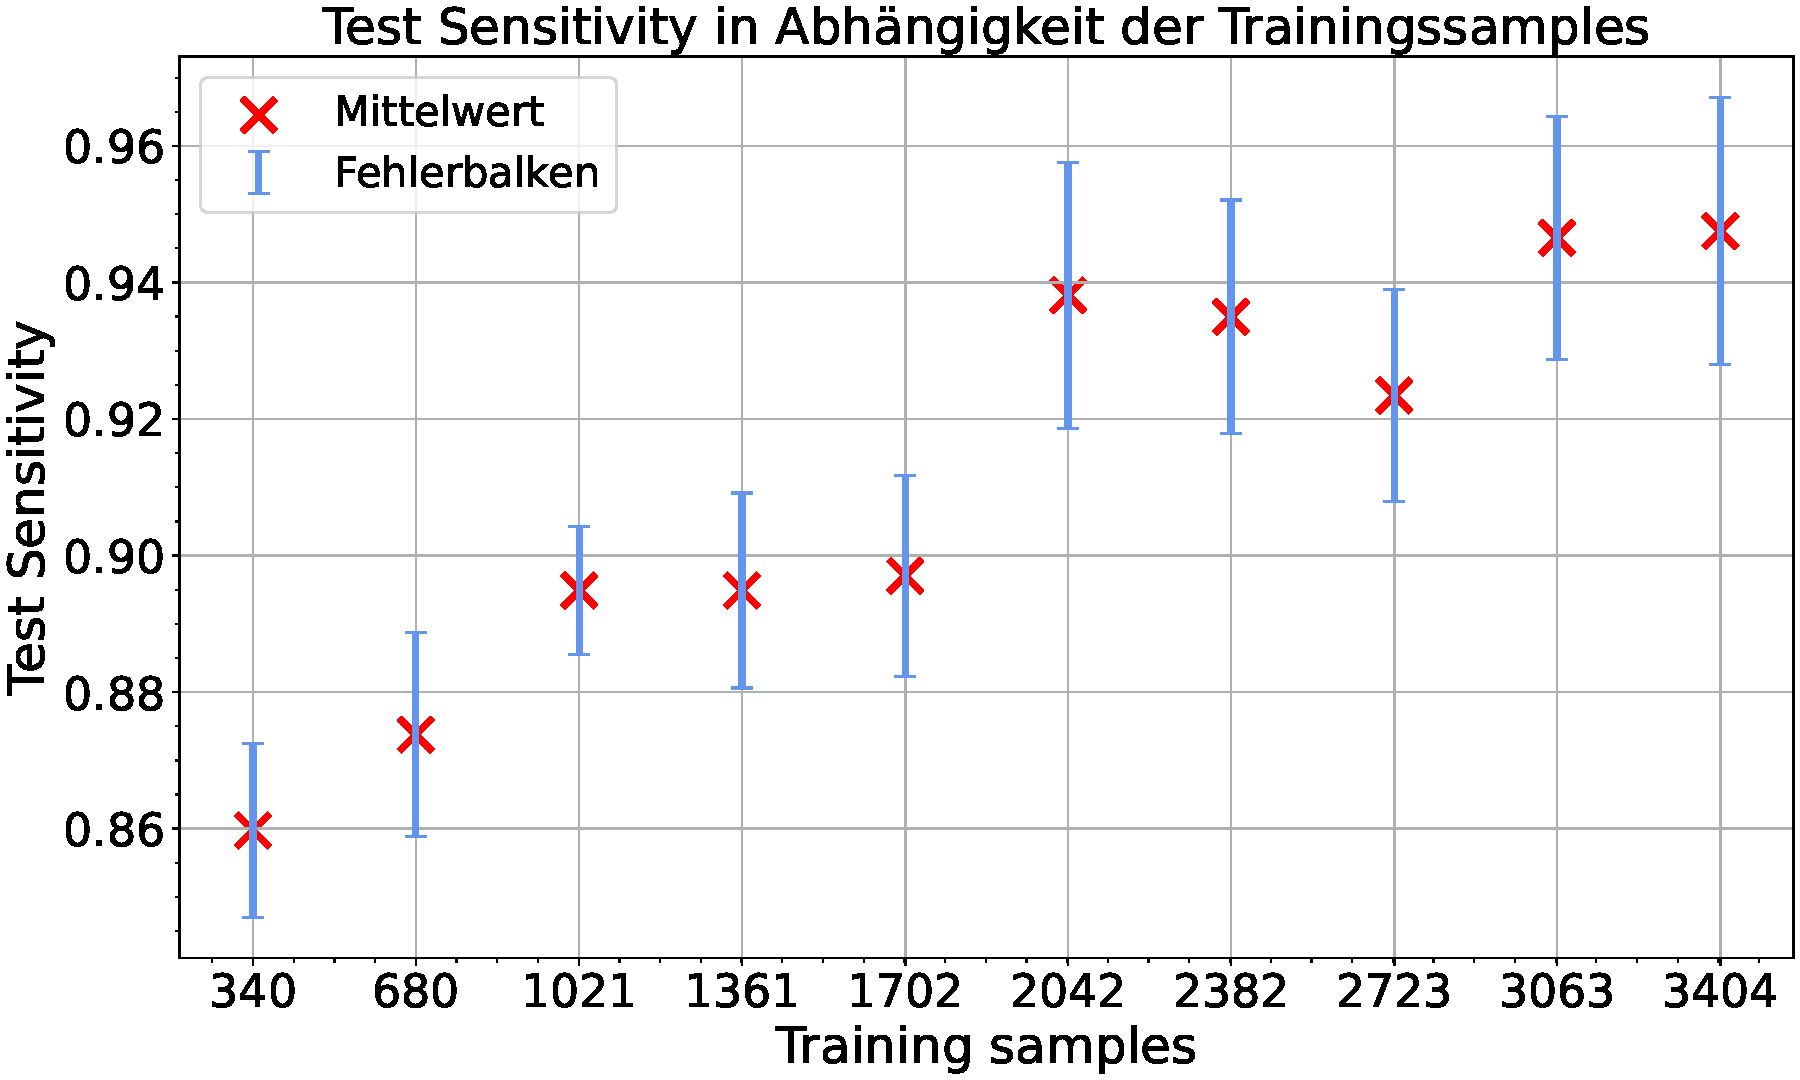
\includegraphics[width=\textwidth]{plots/Augm-Messungen-noTu-Tu_Sensitivity_mean.pdf}
    \caption{Sensitivity}
    \label{fig:augmentation_sensitivity}
  \end{subfigure}
  \begin{subfigure}[b]{0.48\textwidth}
    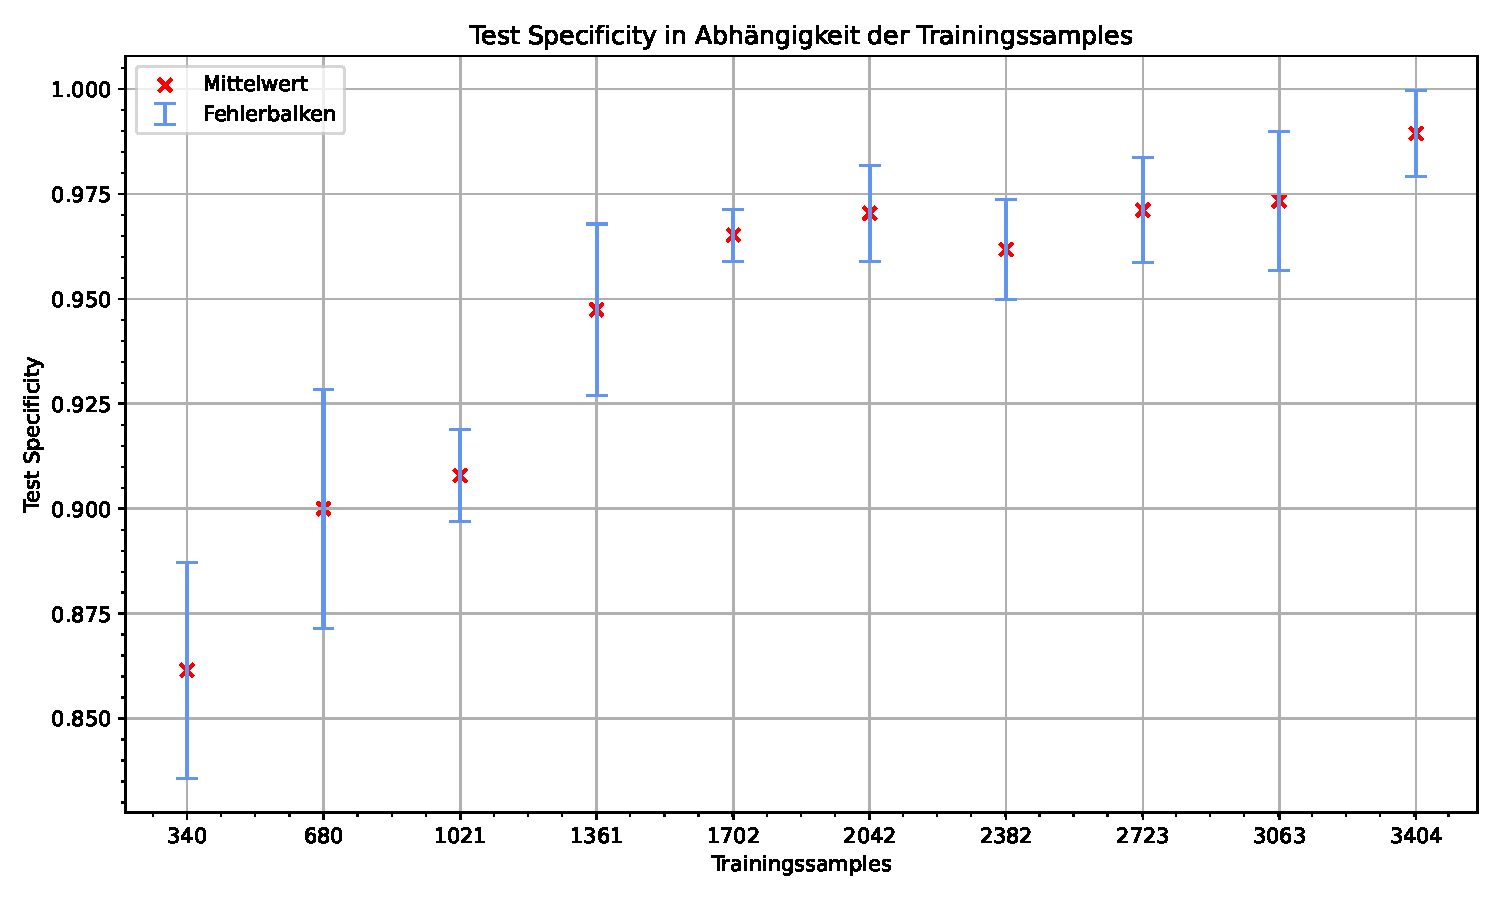
\includegraphics[width=\textwidth]{plots/Augm-Messungen-noTu-Tu_Specificity_mean.pdf}
    \caption{Specificity}
    \label{fig:augmentation_specificity}
  \end{subfigure}
  \caption{Metriken bei Verwendung von Augmentation.}
  \label{fig:augmentation}
\end{figure}

\begin{table}[H]
    \centering
        \begin{tabular}{cccc}
            \toprule
            Trainig sample & Accuracy & Sensitivity & Specificity\\
            \midrule
            340  & $86.0435 \pm 0.6923$ & $0.8597 \pm 0.0127$ & $0.8615 \pm 0.0257$\\
            680  & $88.4273 \pm 0.7041$ & $0.8738 \pm 0.0150$ & $0.9000 \pm 0.0284$\\
            1021 & $90.0099 \pm 0.6376$ & $0.8949 \pm 0.0093$ & $0.9079 \pm 0.0110$\\
            1361 & $91.5925 \pm 0.9418$ & $0.8949 \pm 0.0143$ & $0.9474 \pm 0.0204$\\
            1702 & $92.4332 \pm 0.8357$ & $0.8970 \pm 0.0147$ & $0.9652 \pm 0.0062$\\
            2042 & $95.1039 \pm 1.0250$ & $0.9381 \pm 0.0195$ & $0.9704 \pm 0.0115$\\
            2382 & $94.5697 \pm 0.9296$ & $0.9350 \pm 0.0171$ & $0.9617 \pm 0.0119$\\
            2723 & $94.2532 \pm 1.1726$ & $0.9234 \pm 0.0155$ & $0.9711 \pm 0.0125$\\
            3063 & $95.7270 \pm 1.4340$ & $0.9465 \pm 0.0178$ & $0.9733 \pm 0.0166$\\
            3404 & $96.4293 \pm 1.4880$ & $0.9475 \pm 0.0195$ & $0.9894 \pm 0.0103$\\
            \bottomrule
        \end{tabular}
  \caption{Mittelwert und Standardabweichung der Metriken bei der Augmentation.}
  \label{tab:}
\end{table}
Die Specificity steigt mit zunehmender Anzahl an Training samples an und erreicht ab 1702 Bildern ein Plateau.
Bei der Sensitivity und Accuracy wird ein Plateau ab 2042 Trainingssamples erreicht.
Die Accuracy steigt dabei konstant an. 
Die Sensitivity steigt bis 1021 samples an und bleibt anschließend relativ konstant und erreicht anschließend das Plateau.

\subsection{Reduzierung der Tumorsamples}

\begin{figure}[H]
  \centering
  \begin{subfigure}[b]{0.48\textwidth}
    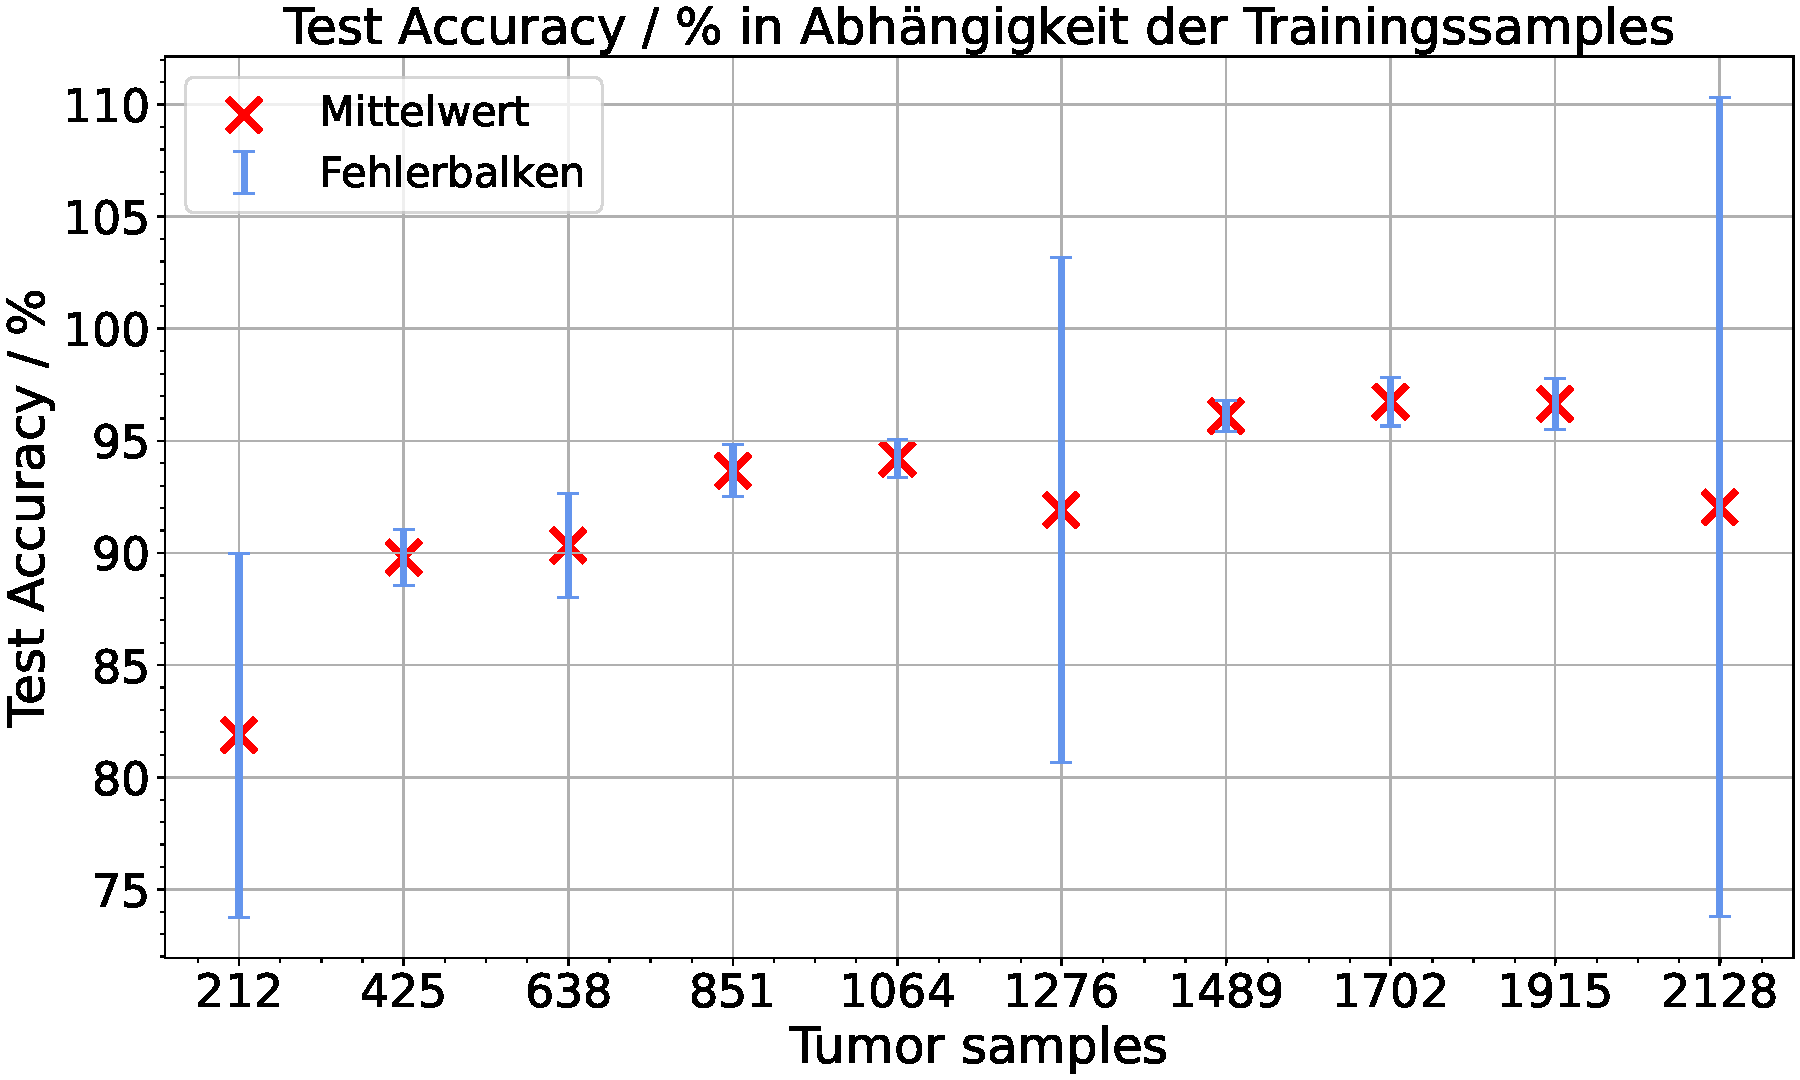
\includegraphics[width=\textwidth]{plots/neu Reduzierung-Tu + Balance_Accuracy_mean.pdf}
    \caption{Accuracy}
    \label{fig:reduzierung_tu_accuracy}
  \end{subfigure}
  \begin{subfigure}[b]{0.48\textwidth}
    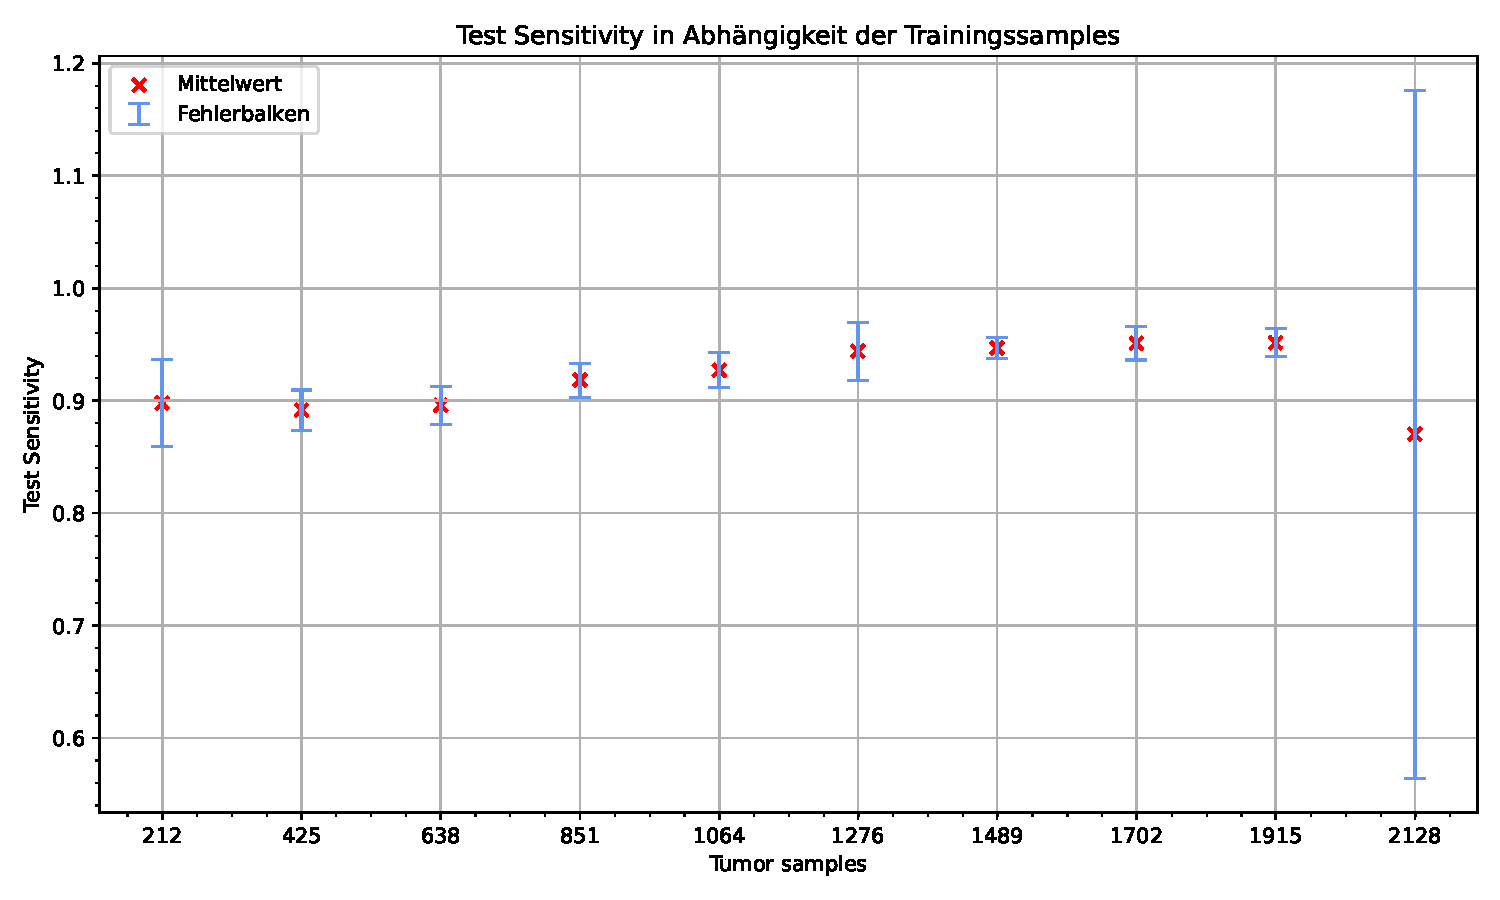
\includegraphics[width=\textwidth]{plots/neu Reduzierung-Tu + Balance_Sensitivity_mean.pdf}
    \caption{Sensitivity}
    \label{fig:reduzierung_tu_sensitivity}
  \end{subfigure}
  \begin{subfigure}[b]{0.48\textwidth}
    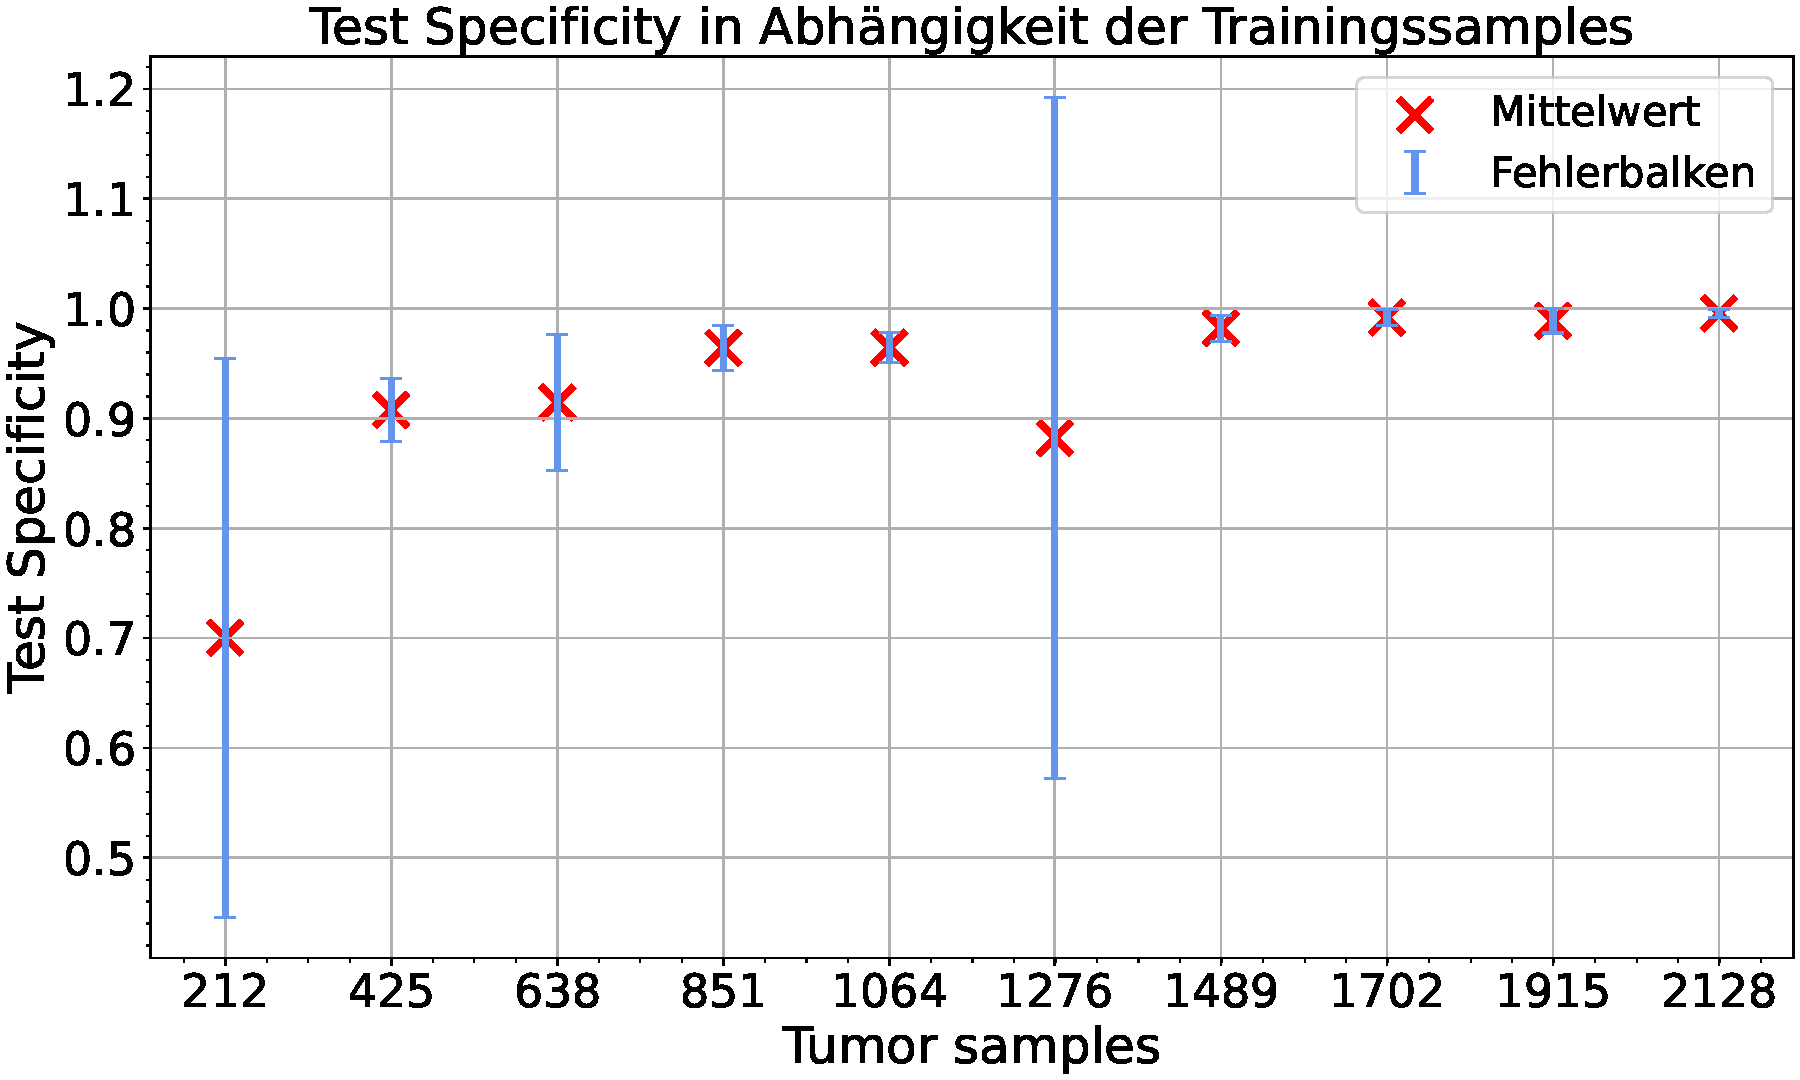
\includegraphics[width=\textwidth]{plots/neu Reduzierung-Tu + Balance_Specificity_mean.pdf}
    \caption{Specificity}
    \label{fig:reduzierung_tu_specificity}
  \end{subfigure}
  \caption{Metriken bei Reduktion der Tumor-Trainingsbeispiele mit Ausbalancierung}
  \label{fig:reduzierung_tumorsamples}
\end{figure}

\begin{table}[H]
    \centering
        \begin{tabular}{cccc}
            \toprule
            Trainig sample & Accuracy & Sensitivity & Specificity\\
            \midrule
            212  & $81.8694 \pm 8.1081$ & $0.8979 \pm 0.0389$ & $0.7002 \pm 0.2544$\\
            425  & $89.8022 \pm 1.2611$ & $0.8916 \pm 0.0179$ & $0.9077 \pm 0.0285$\\
            638  & $90.3363 \pm 2.3230$ & $0.8959 \pm 0.0170$ & $0.9146 \pm 0.0622$\\
            851  & $93.6696 \pm 1.1535$ & $0.9183 \pm 0.0151$ & $0.9642 \pm 0.0203$\\
            1064 & $94.2038 \pm 0.8486$ & $0.9271 \pm 0.0156$ & $0.9644 \pm 0.0135$\\
            1276 & $91.9189 \pm 11.273$ & $0.9441 \pm 0.0258$ & $0.8820 \pm 0.3100$\\
            1489 & $96.1029 \pm 0.6919$ & $0.9469 \pm 0.0095$ & $0.9822 \pm 0.0118$\\
            1702 & $96.7458 \pm 1.0820$ & $0.9512 \pm 0.0150$ & $0.9919 \pm 0.0069$\\
            1915 & $96.6469 \pm 1.1234$ & $0.9515 \pm 0.0124$ & $0.9889 \pm 0.0111$\\
            2128 & $92.0376 \pm 18.269$ & $0.8701 \pm 0.3058$ & $0.9956 \pm 0.0036$\\
            \bottomrule
        \end{tabular}
  \caption{Mittelwert und Standardabweichung der Metriken bei der Reduzierung von Tumor Klasse.}
  \label{tab:}
\end{table}

\section{Klassifizierung zwischen Glioma und Meningioma}

\subsection{Hyperparameter}
\begin{figure}[htbp]
  \centering
  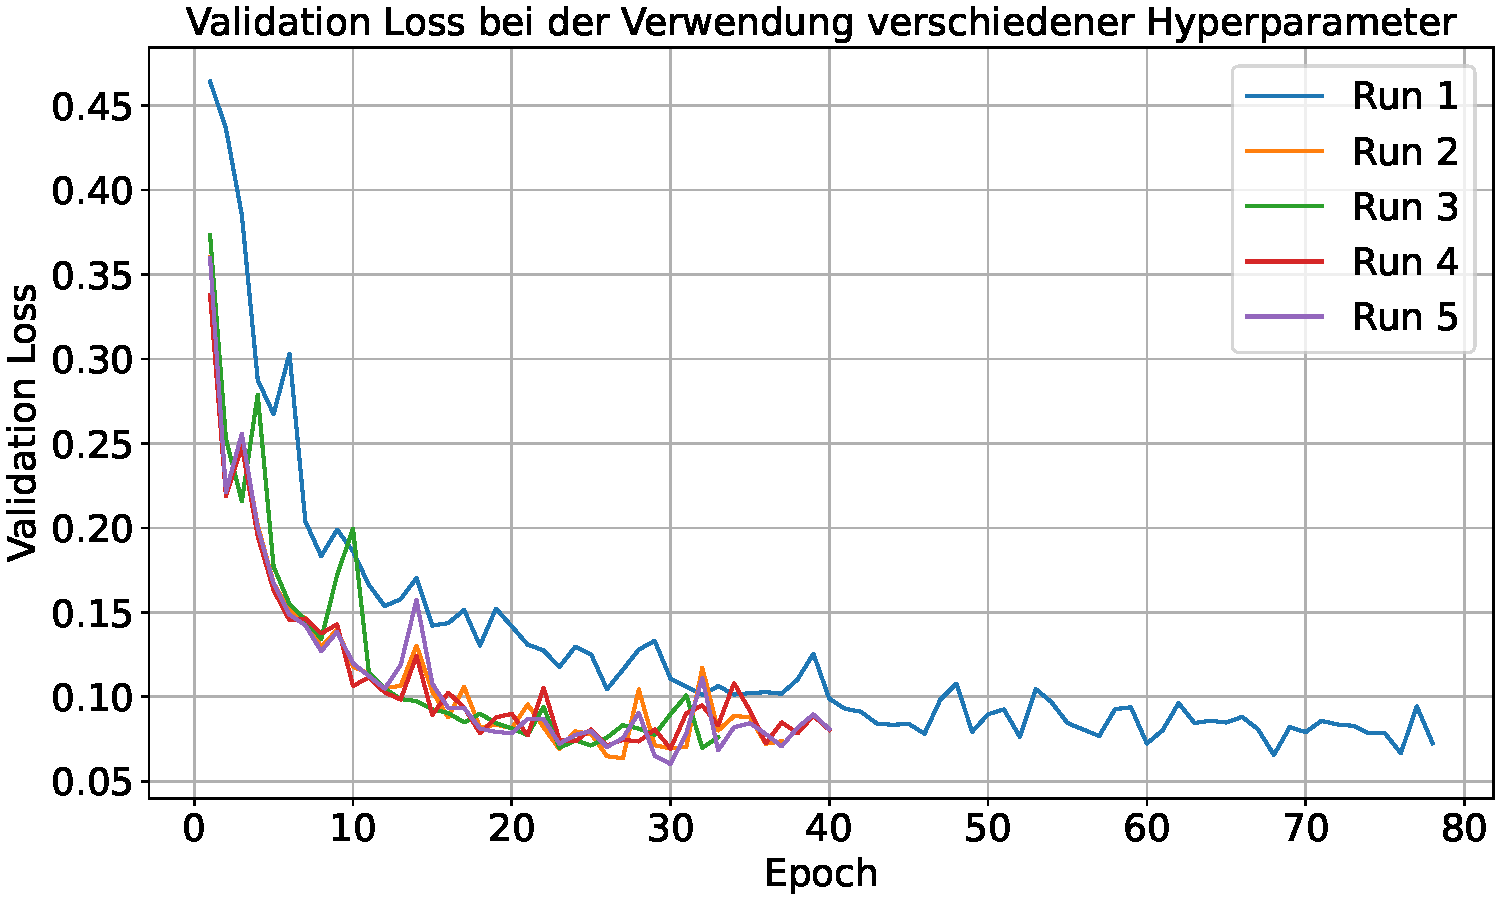
\includegraphics[scale=0.4]{plots/Val_loss_Gli_Men.pdf}
  \caption{Darstellung des Validierungs Loss bei der Verwendung verschiedener Hyperparameter.}
  \label{fig:val_loss gli-men}
\end{figure}

\begin{table}[htbp]
    \centering
    \resizebox{\textwidth}{!}{%
        \begin{tabular}{cccccccc}
            \toprule
            Runs & Batch Größe & Lernrate & Dropout & Validation Loss & Accuracy/$\%$ & Sensitivity & Specificity \\
            \midrule
            1 & 128 & 0.01  & 0.55 & 0.18943 & 92.29323 & 0.95402 & 0.89299 \\
            2 & 64  & 0.005 & 0.3  & 0.22499 & 93.23308 & 0.96935 & 0.89668 \\
            3 & 16  & 0.0005& 0.55 & 0.23146 & 93.98496 & 0.9272  & 0.95203 \\
            4 & 16  & 0.005 & 0.5  & 0.23453 & 92.66917 & 0.95402 & 0.90037 \\
            5 & 16  & 0.0005& 0.5  & 0.23829 & 93.42105 & 0.94253 & 0.9262 \\
            \bottomrule
        \end{tabular}
    }
  \caption{.}
  \label{tab:hyperp gli men }
\end{table}

\subsection{Reduzierung der Trainingsdaten}

\begin{figure}[htbp]
  \centering
  \begin{subfigure}[b]{0.48\textwidth}
    \centering
    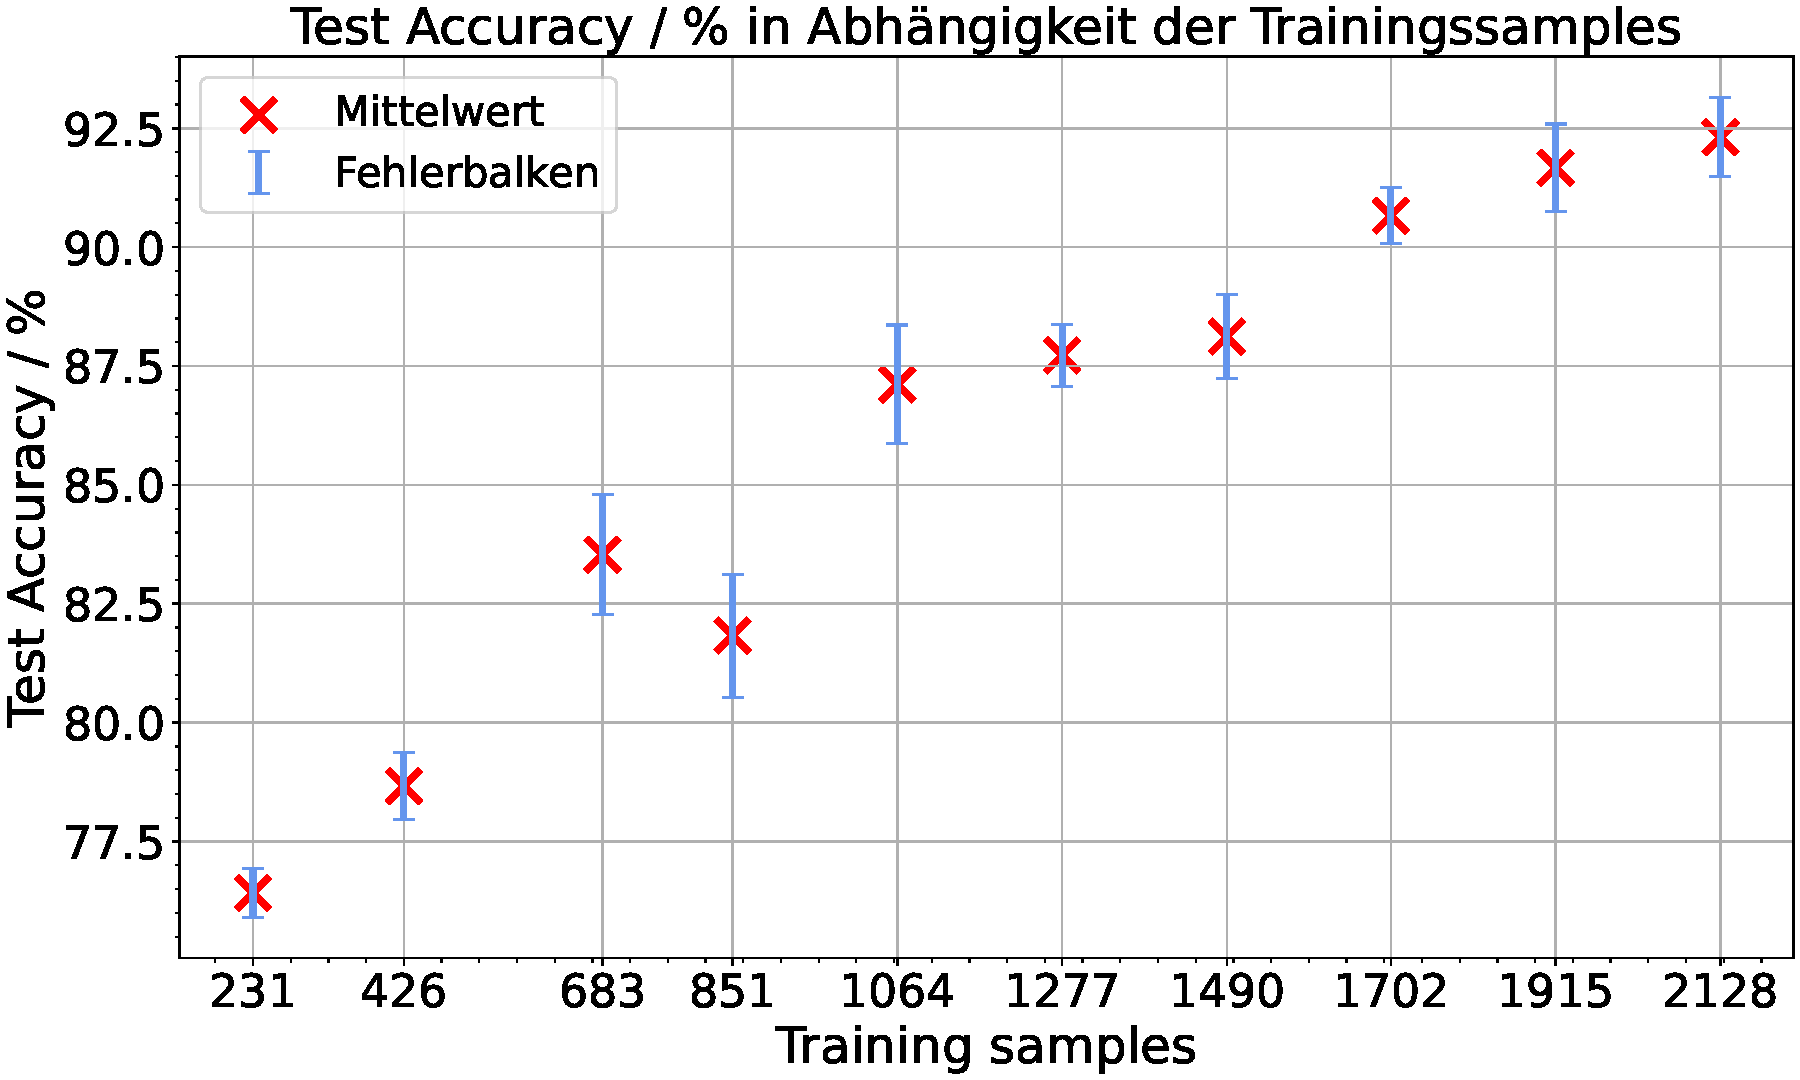
\includegraphics[width=\textwidth]{plots/3-Messungen-Gli-Men_Accuracy_mean.pdf}
    \caption{Accuracy}
    \label{fig:gli-men-acc}
  \end{subfigure}
  \begin{subfigure}[b]{0.48\textwidth}
    \centering
    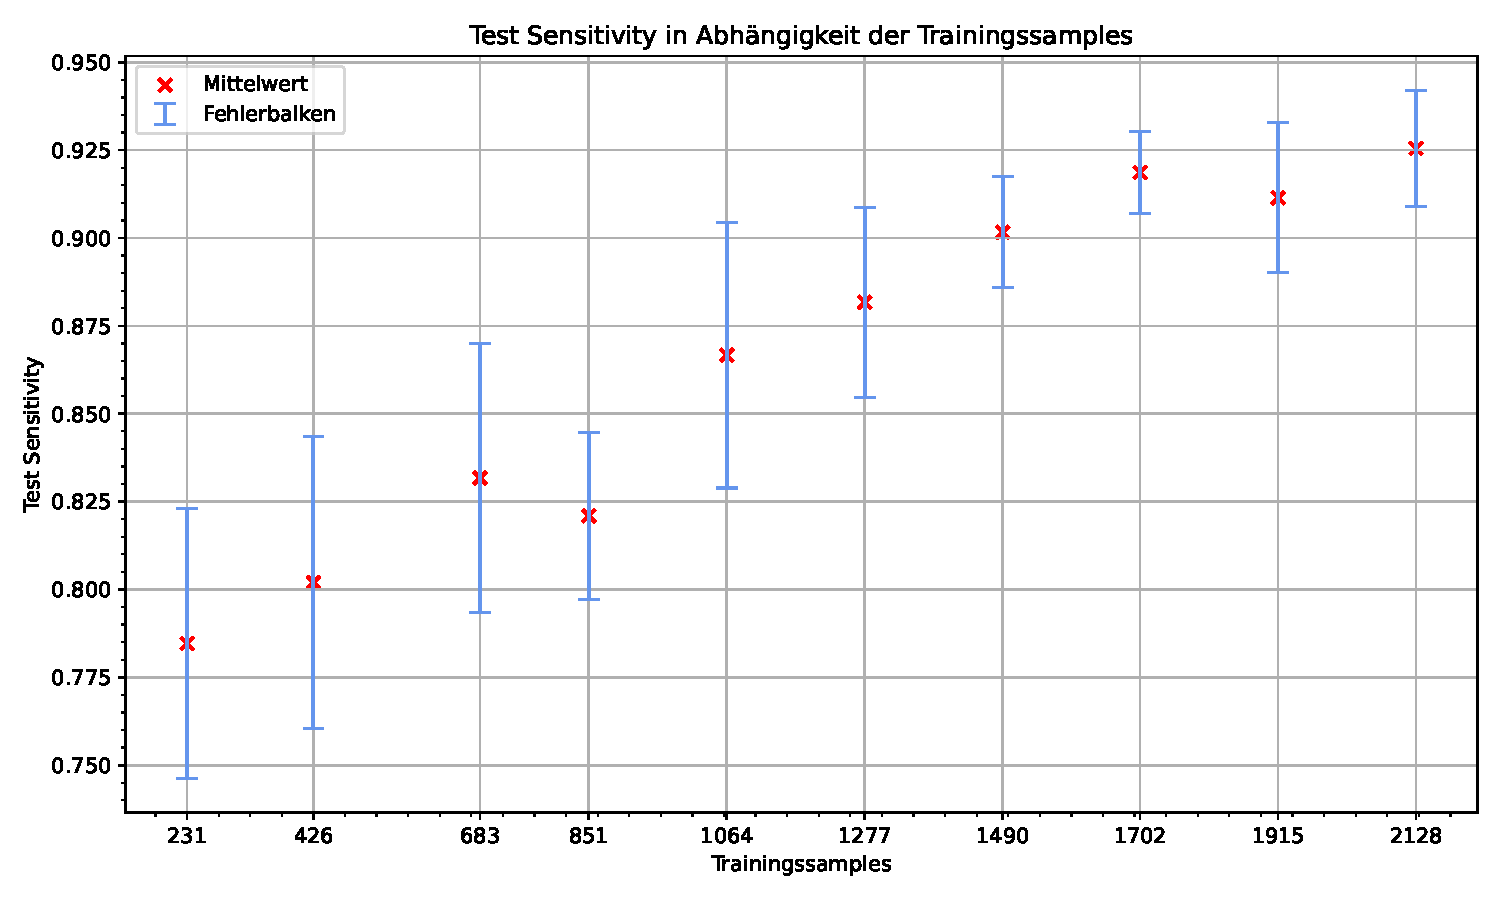
\includegraphics[width=\textwidth]{plots/3-Messungen-Gli-Men_Sensitivity_mean.pdf}
    \caption{Sensitivität}
    \label{fig:gli-men-sens}
  \end{subfigure}
  \begin{subfigure}[b]{0.48\textwidth}
    \centering
    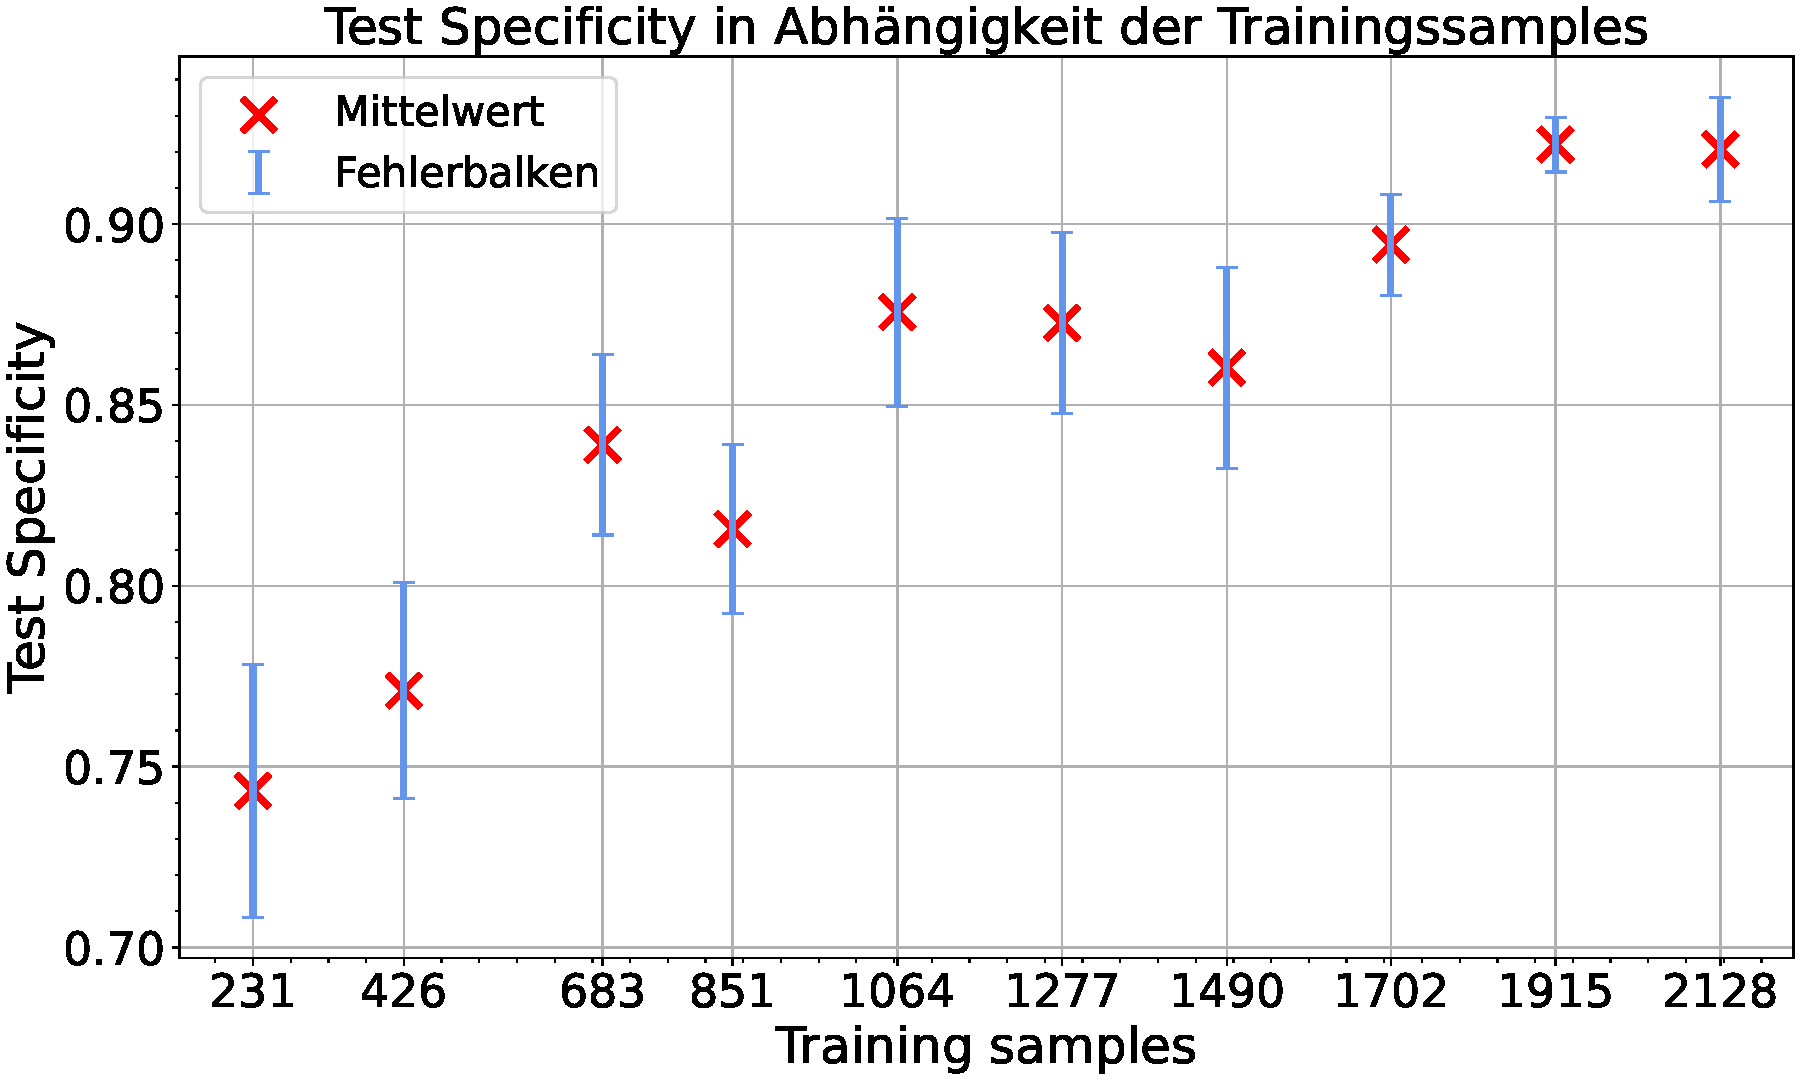
\includegraphics[width=\textwidth]{plots/3-Messungen-Gli-Men_Specificity_mean.pdf}
    \caption{Spezifität}
    \label{fig:gli-men-spec}
  \end{subfigure}
  \caption{}
  \label{fig:gli-men-reduktion}
\end{figure}

\subsection{Augmentation}

\begin{figure}[htbp]
  \centering
  \begin{subfigure}[b]{0.48\textwidth}
    \centering
    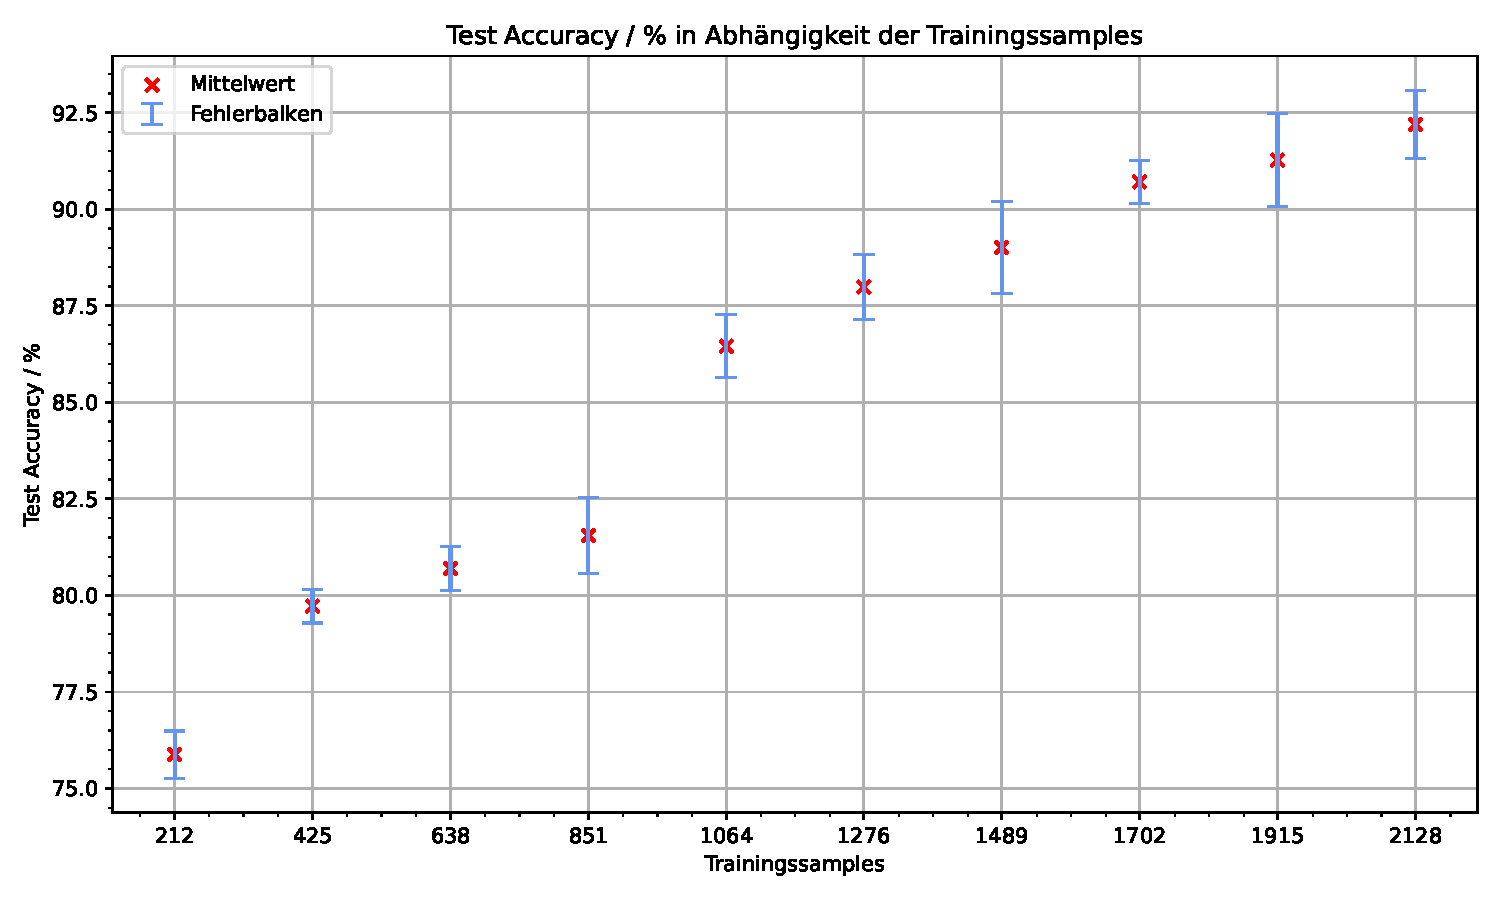
\includegraphics[width=\textwidth]{plots/Augm-Gli-Men_Accuracy_mean.pdf}
    \caption{Accuracy}
    \label{fig:augm-acc}
  \end{subfigure}
  \begin{subfigure}[b]{0.48\textwidth}
    \centering
    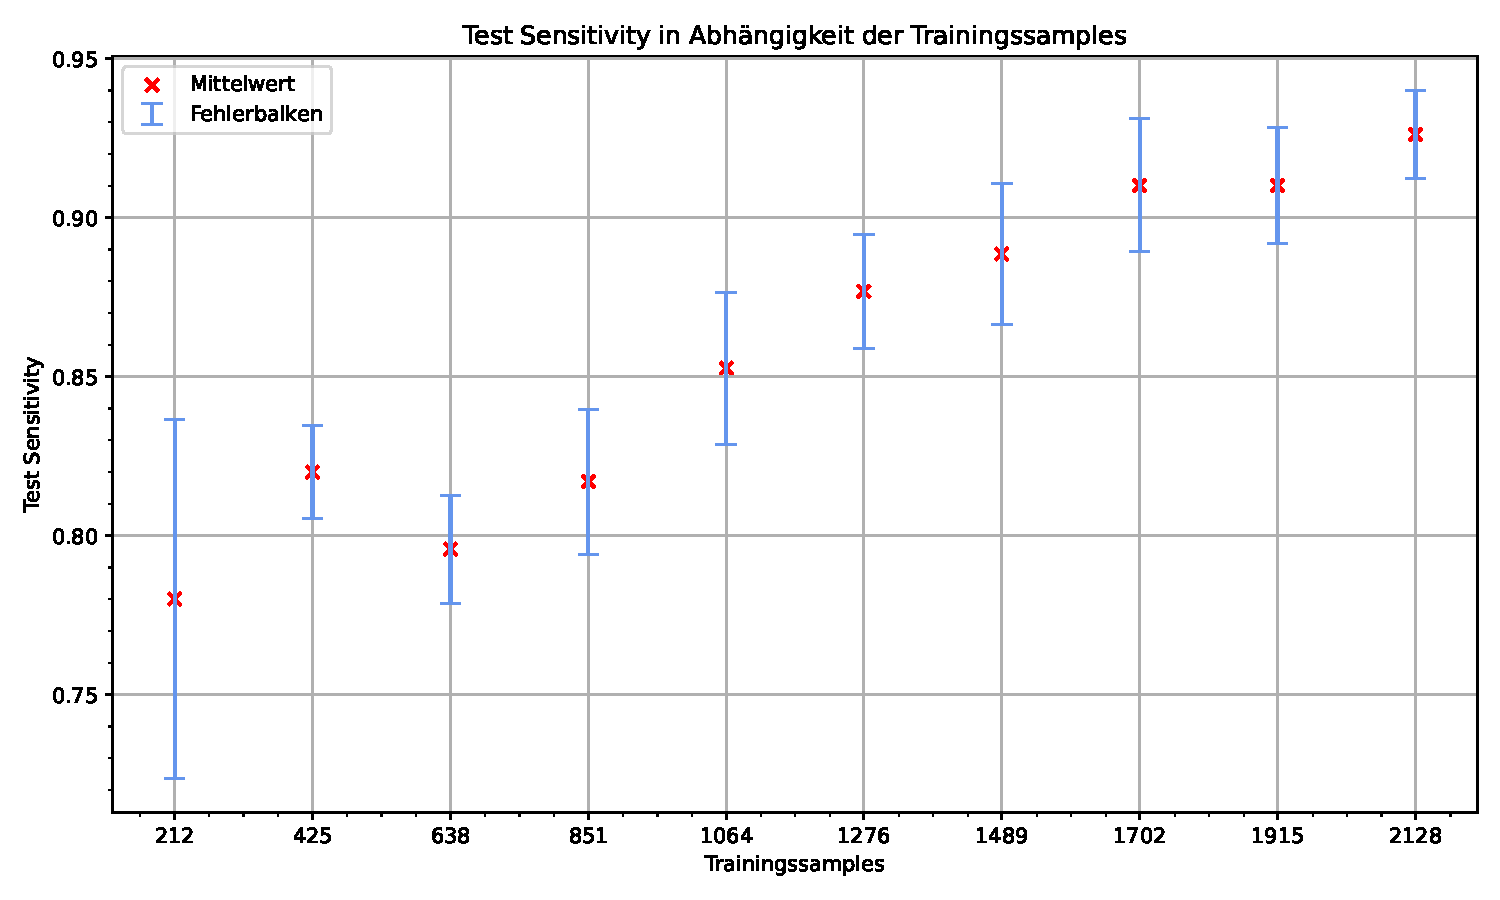
\includegraphics[width=\textwidth]{plots/Augm-Gli-Men_Sensitivity_mean.pdf}
    \caption{Sensitivität}
    \label{fig:augm-sens}
  \end{subfigure}
  \begin{subfigure}[b]{0.48\textwidth}
    \centering
    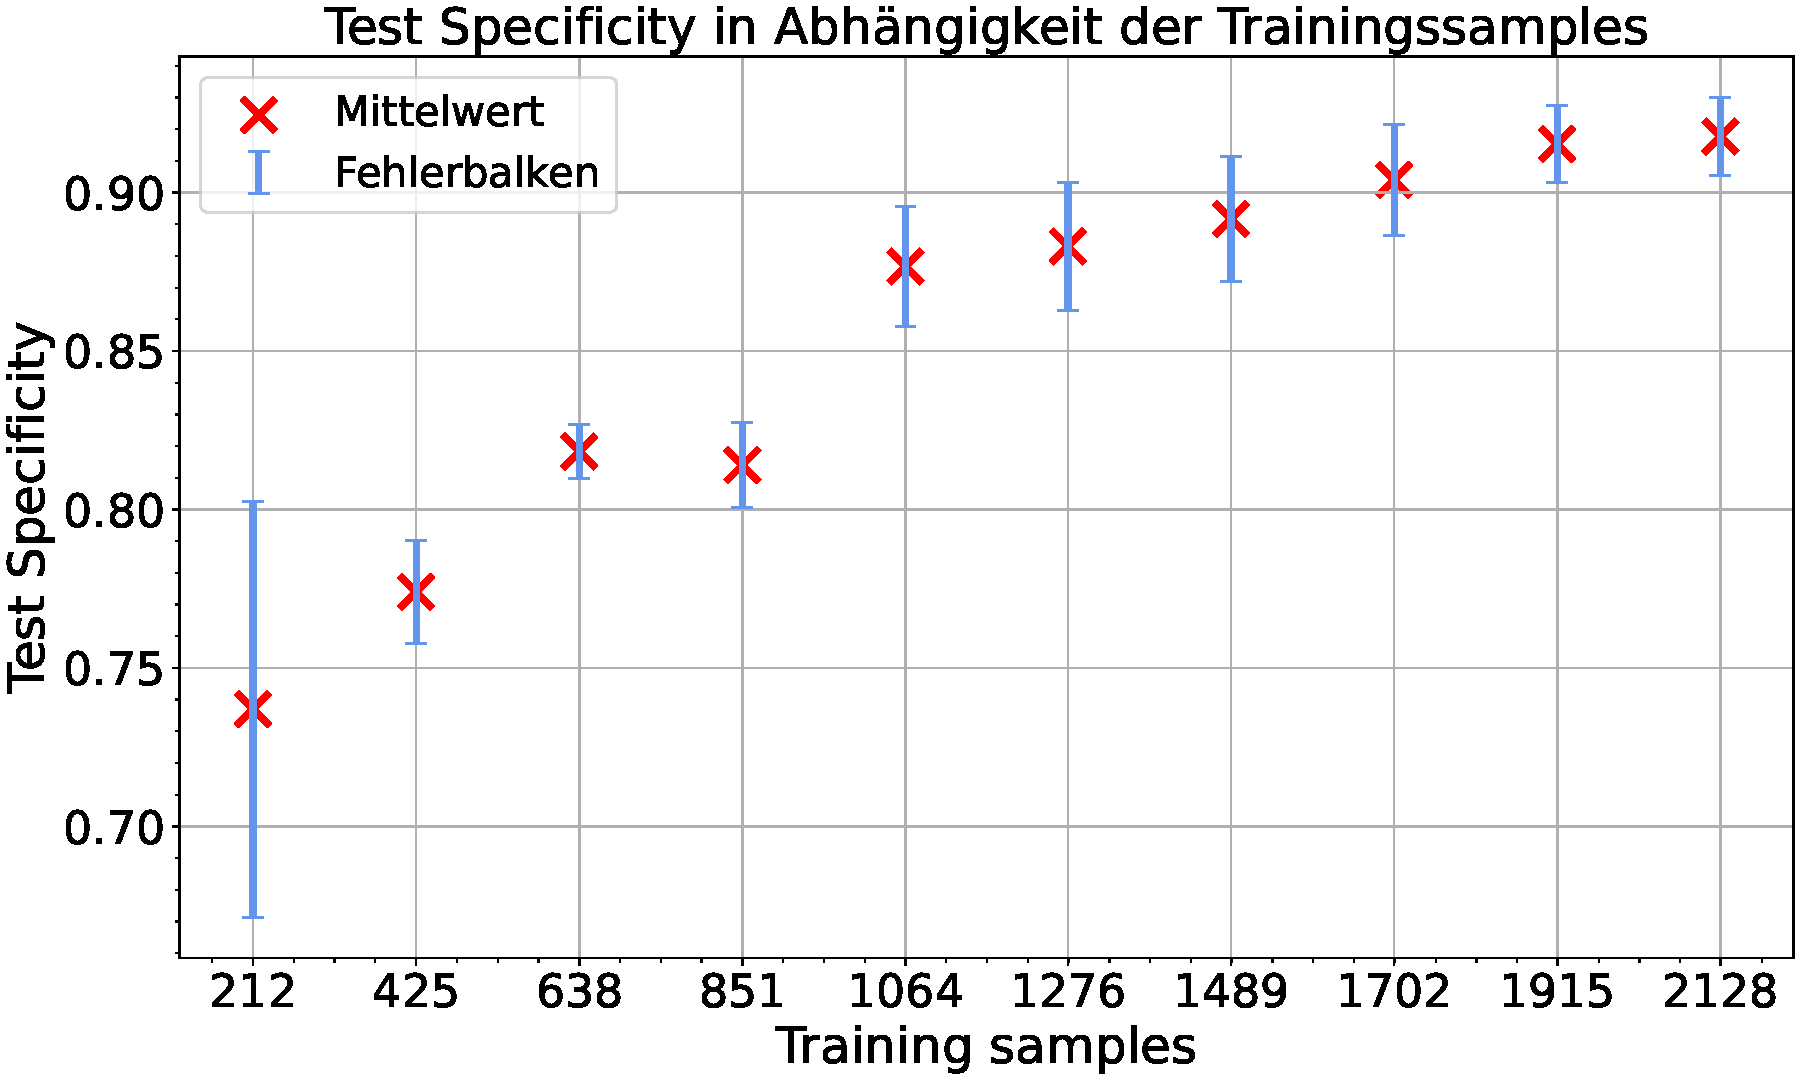
\includegraphics[width=\textwidth]{plots/Augm-Gli-Men_Specificity_mean.pdf}
    \caption{Spezifität}
    \label{fig:augm-spec}
  \end{subfigure}
  \caption{.}
  \label{fig:gli-men-augm}
\end{figure}


\subsection{Reduzierung der Gliom-Proben}
\begin{figure}[htbp]
  \centering
  \begin{subfigure}[b]{0.48\textwidth}
    \centering
    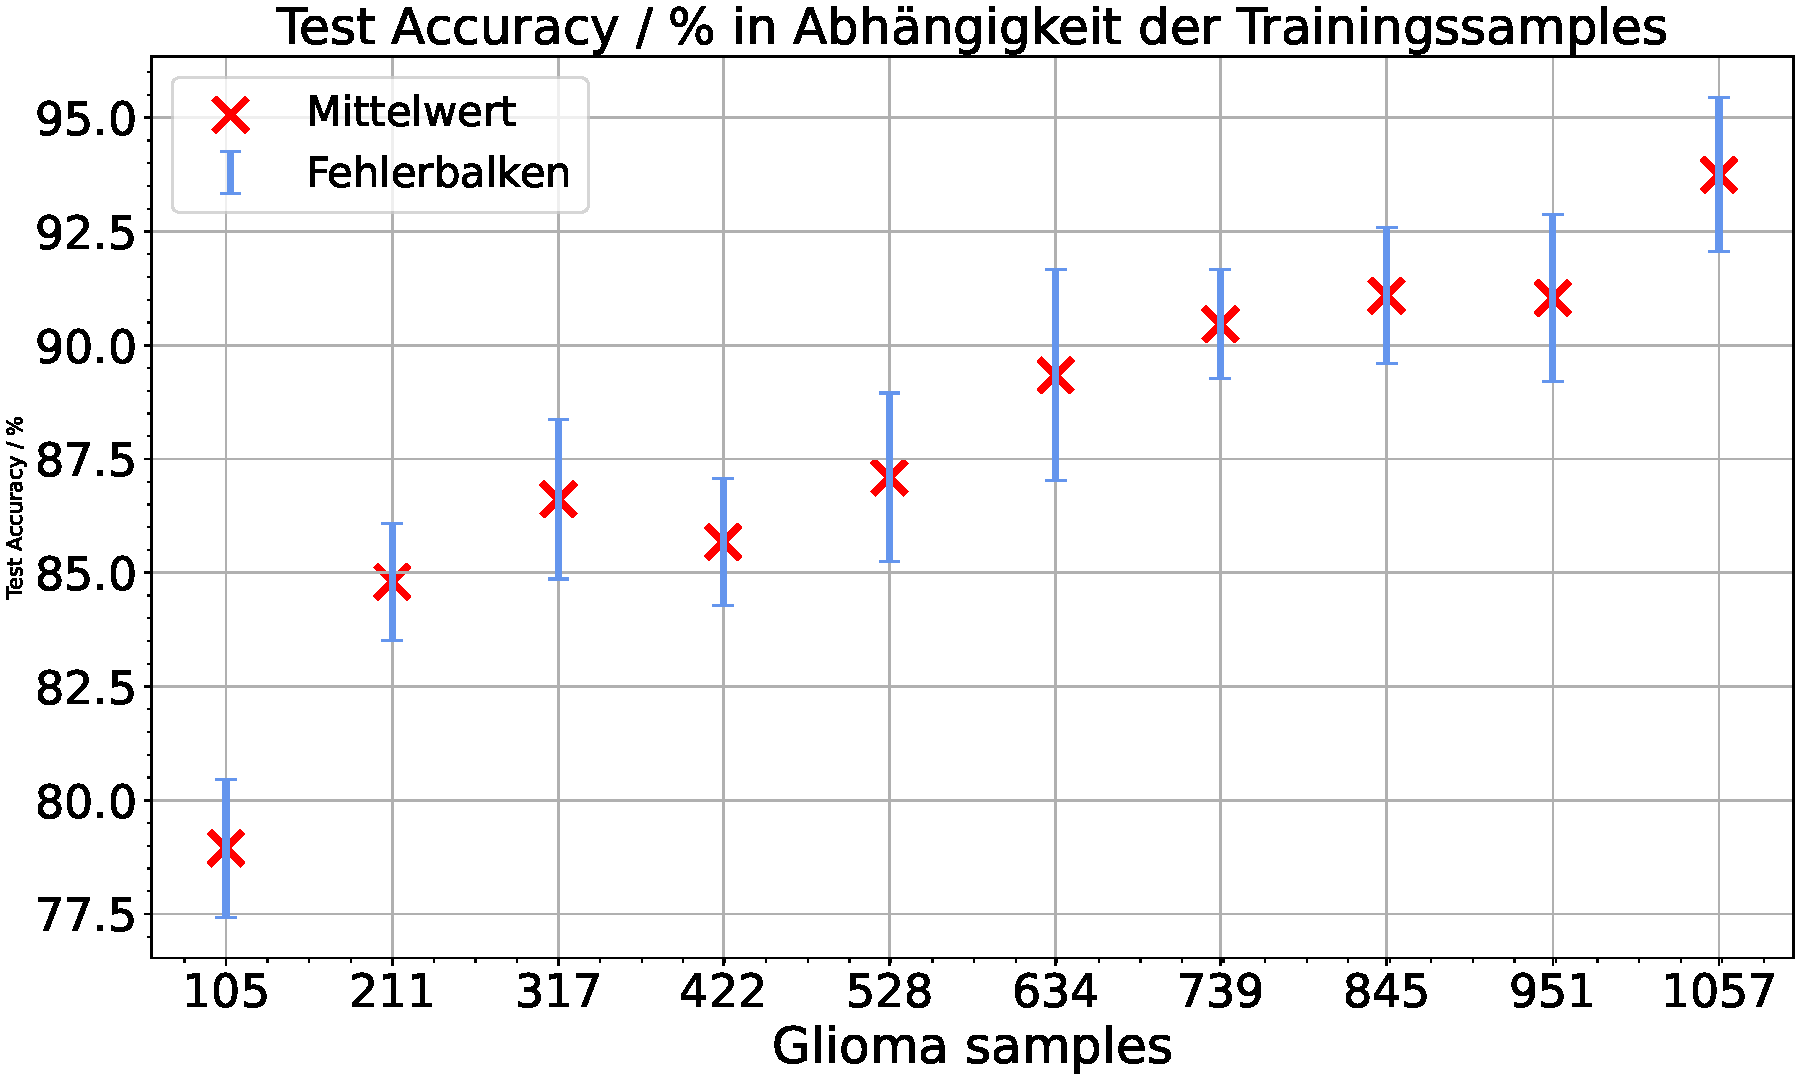
\includegraphics[width=\textwidth]{plots/Reduzierung-Gli + Balnce_Accuracy_mean.pdf}
    \caption{Accuracy}
    \label{fig:gli-red-acc}
  \end{subfigure}
  \begin{subfigure}[b]{0.48\textwidth}
    \centering
    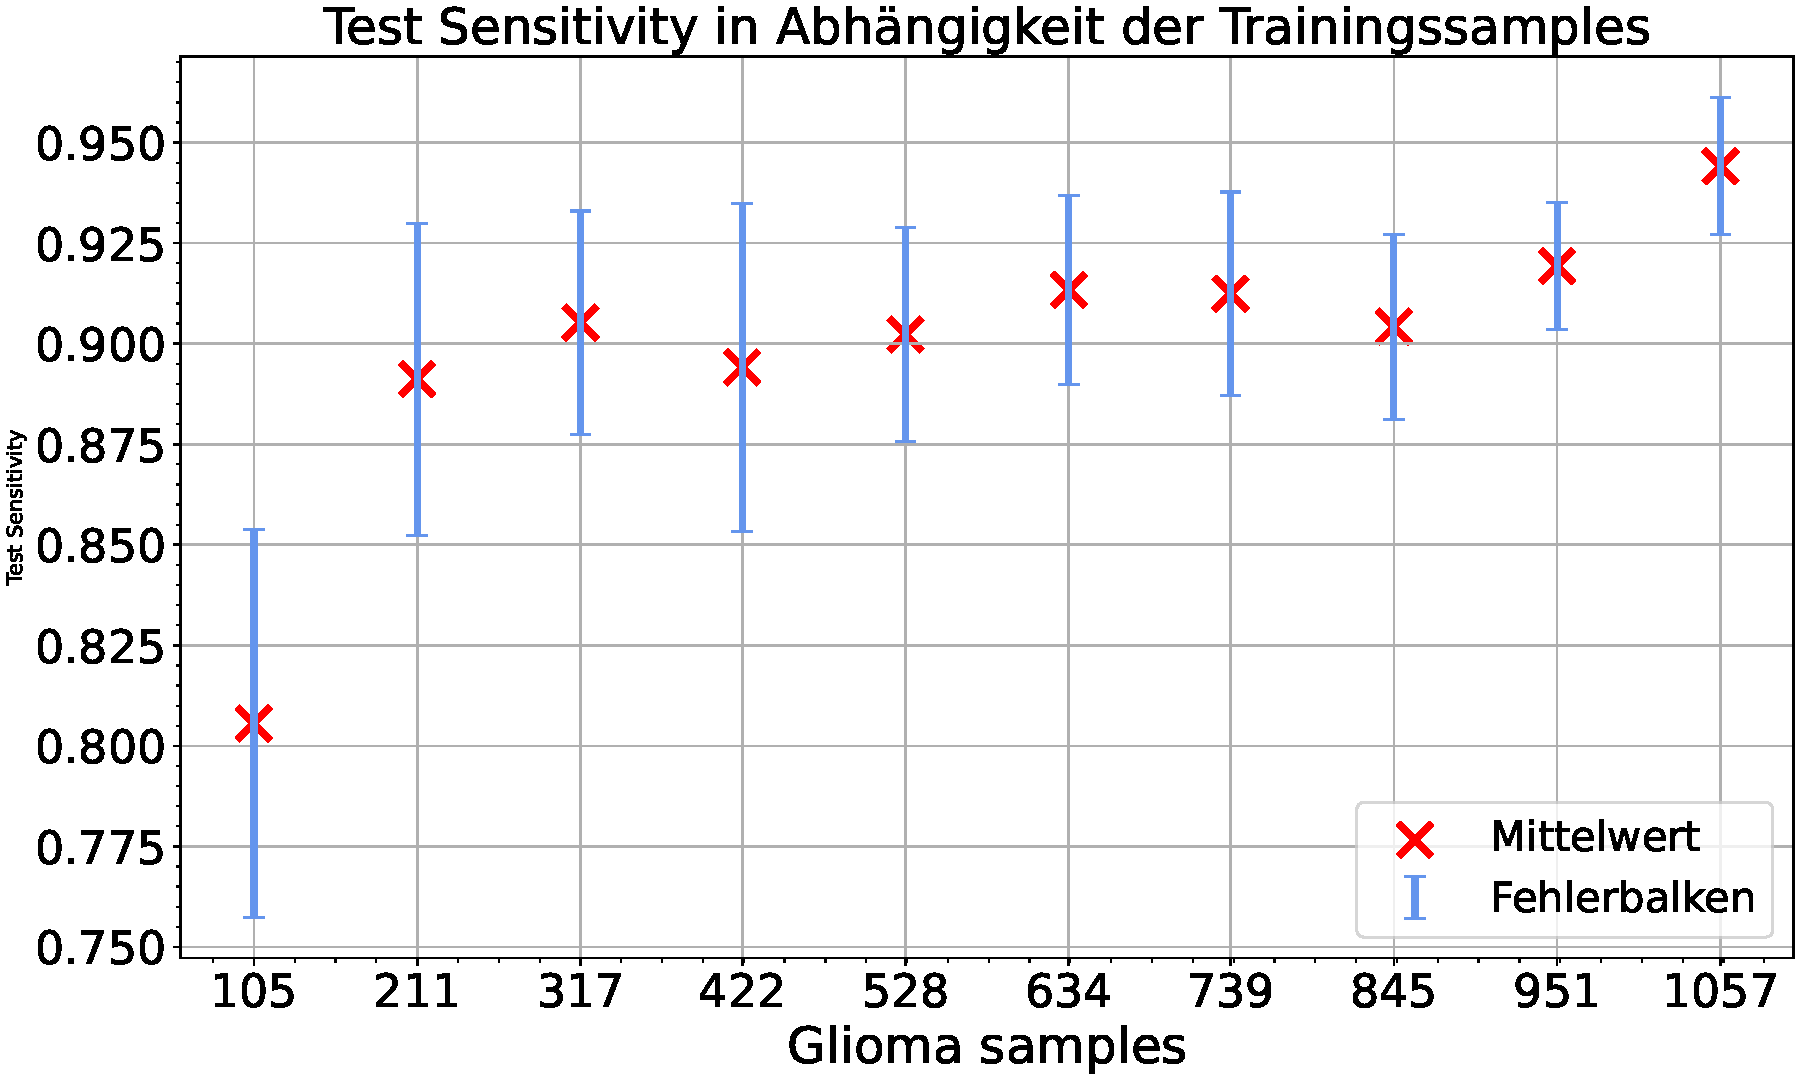
\includegraphics[width=\textwidth]{plots/Reduzierung-Gli + Balnce_Sensitivity_mean.pdf}
    \caption{Sensitivität}
    \label{fig:gli-red-sens}
  \end{subfigure}
  \begin{subfigure}[b]{0.48\textwidth}
    \centering
    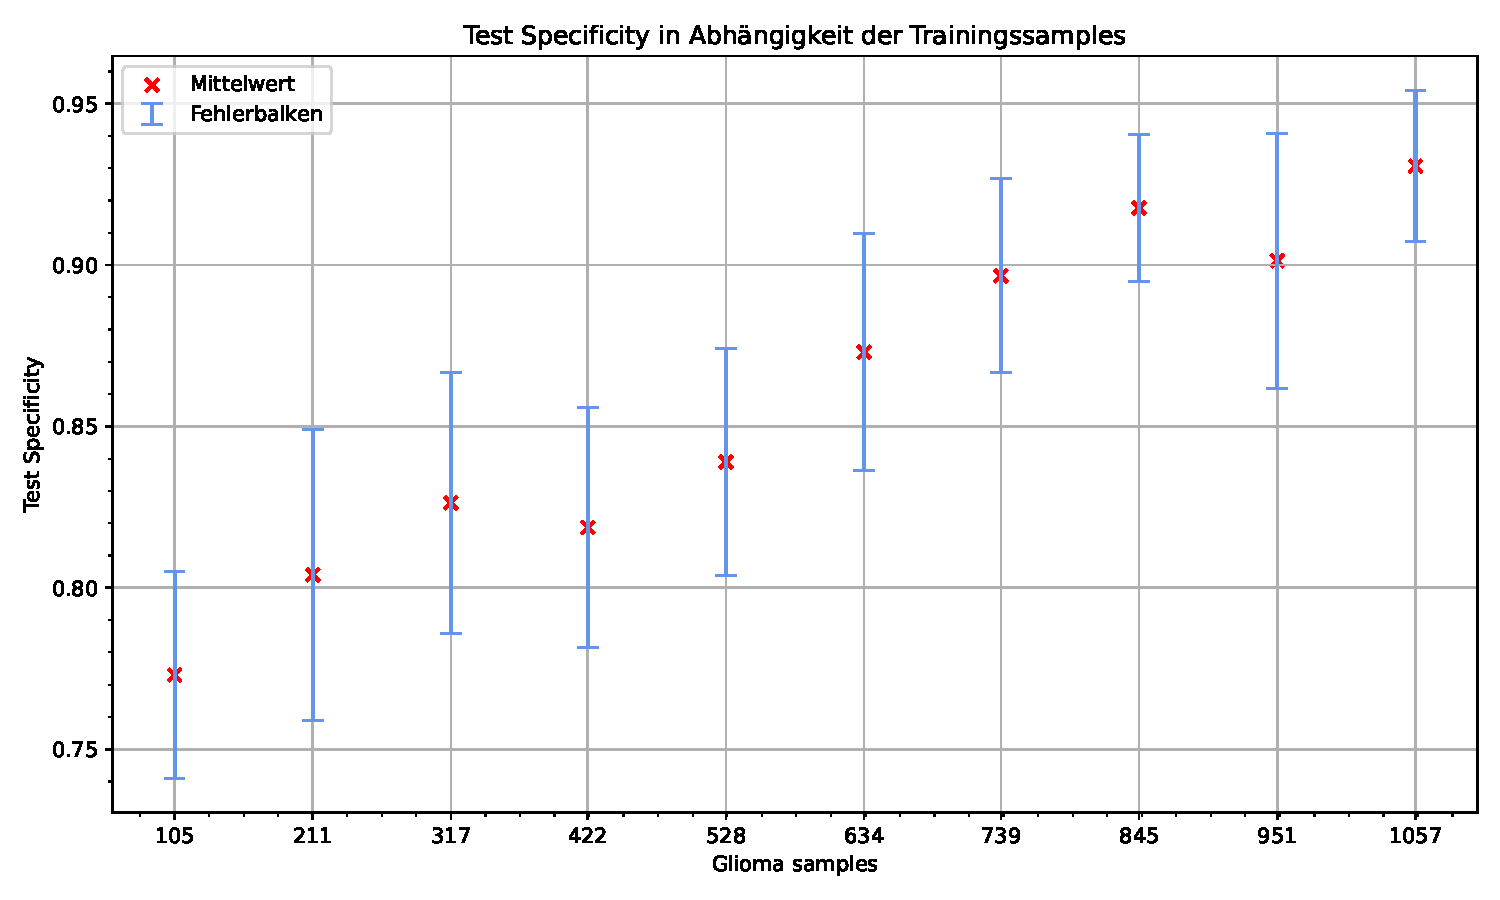
\includegraphics[width=\textwidth]{plots/Reduzierung-Gli + Balnce_Specificity_mean.pdf}
    \caption{Spezifität}
    \label{fig:gli-red-spec}
  \end{subfigure}
  \caption{.}
  \label{fig:gli-men-gliored}
\end{figure}


